\textbf{Задание}

Промоделировать систему, состоящую из генератора, памяти и обслуживающего аппарата. Генератор подает сообщения, распределенные по равномерному закону, они приходят в память и выбираются на обработку по закону Пуассона. Количество заявок задано. 
Предусмотреть случай, когда обработанная заявка возвращаетсяобратно в очередь. Определить оптимальную длину очереди, при которойне будет потерянных сообщений. Реализовать двумя способами: используяпошаговый и событийный подходы

\textbf{Результаты работы программы}
$N = 10000$

$a = 0$

$b = 8$

$\Delta t = 0.01$

\begin{figure}[!htb]
    \begin{minipage}{0.55\textwidth}
      \centering
      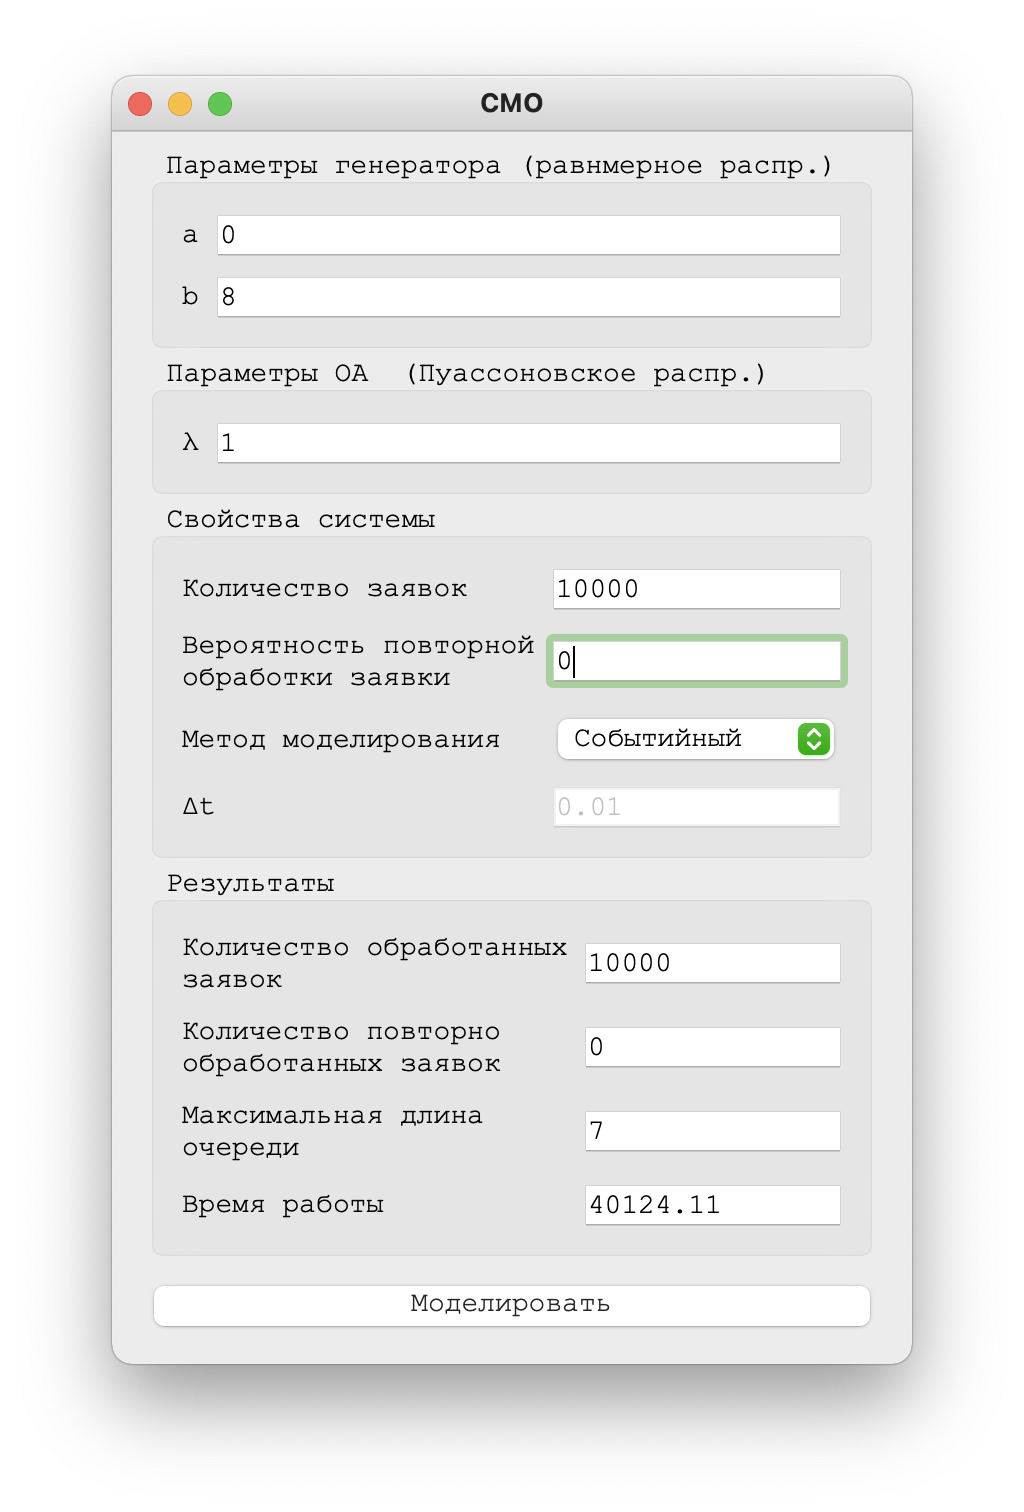
\includegraphics[width=1\linewidth]{1-0-s}
    \end{minipage}\hfill
    \begin{minipage}{0.55\textwidth}
      \centering
      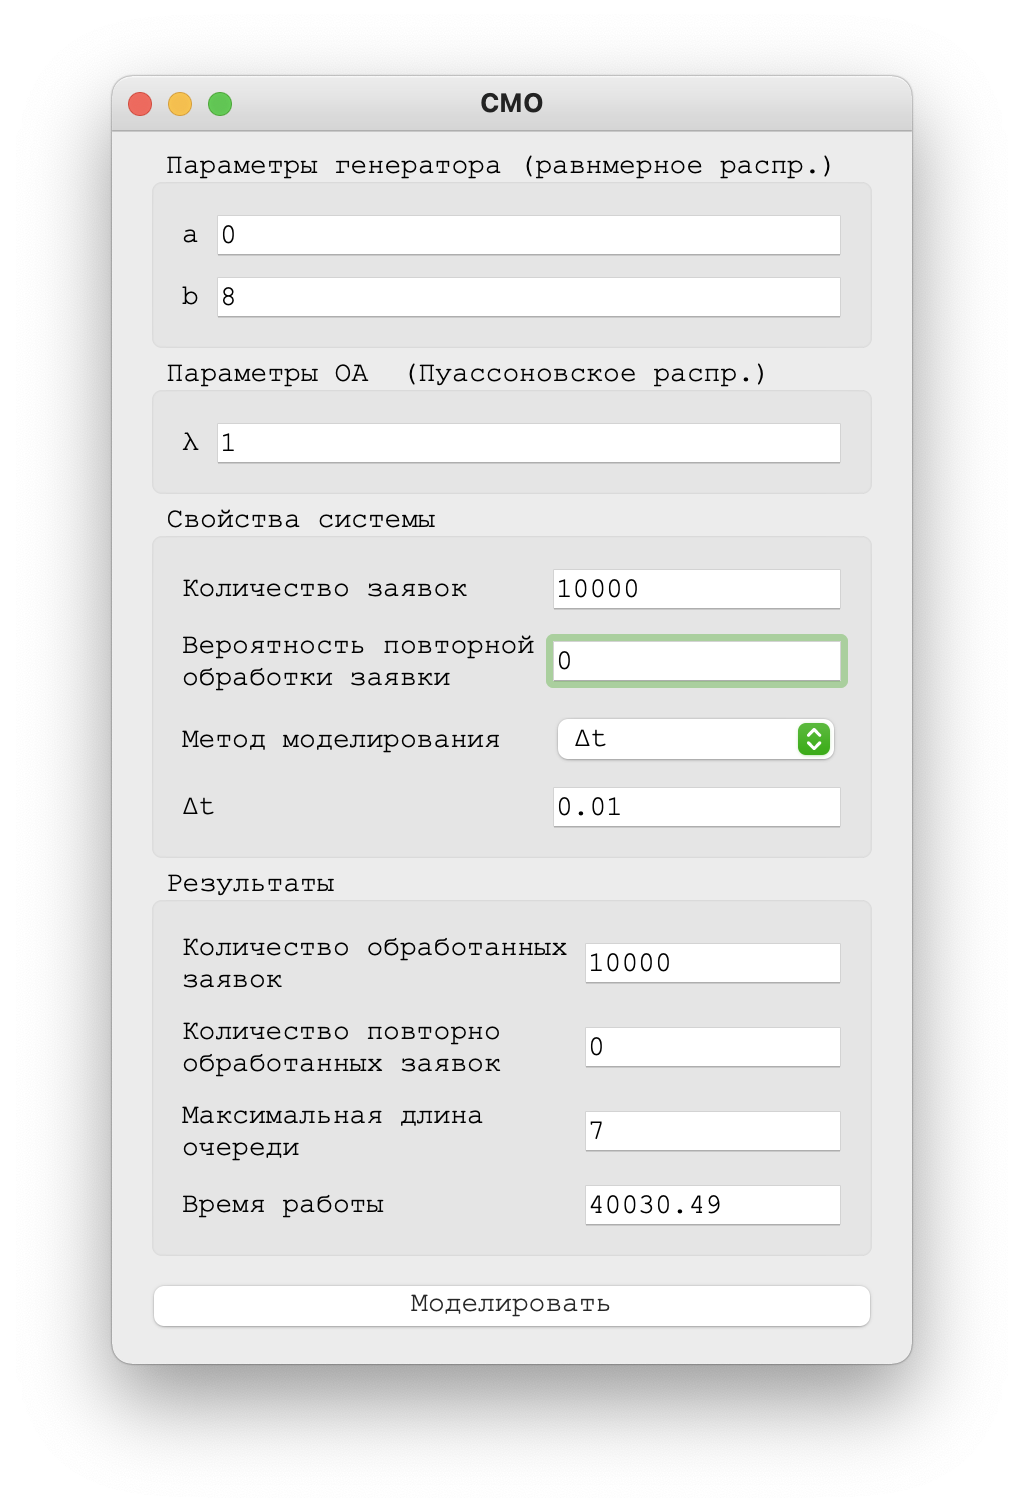
\includegraphics[width=1\linewidth]{1-0-t}
    \end{minipage}
    \caption{Пример работы программы при $p$ = 0 , $\lambda = 1$}
 \end{figure}


 \begin{figure}[!htb]
    \begin{minipage}{0.55\textwidth}
      \centering
      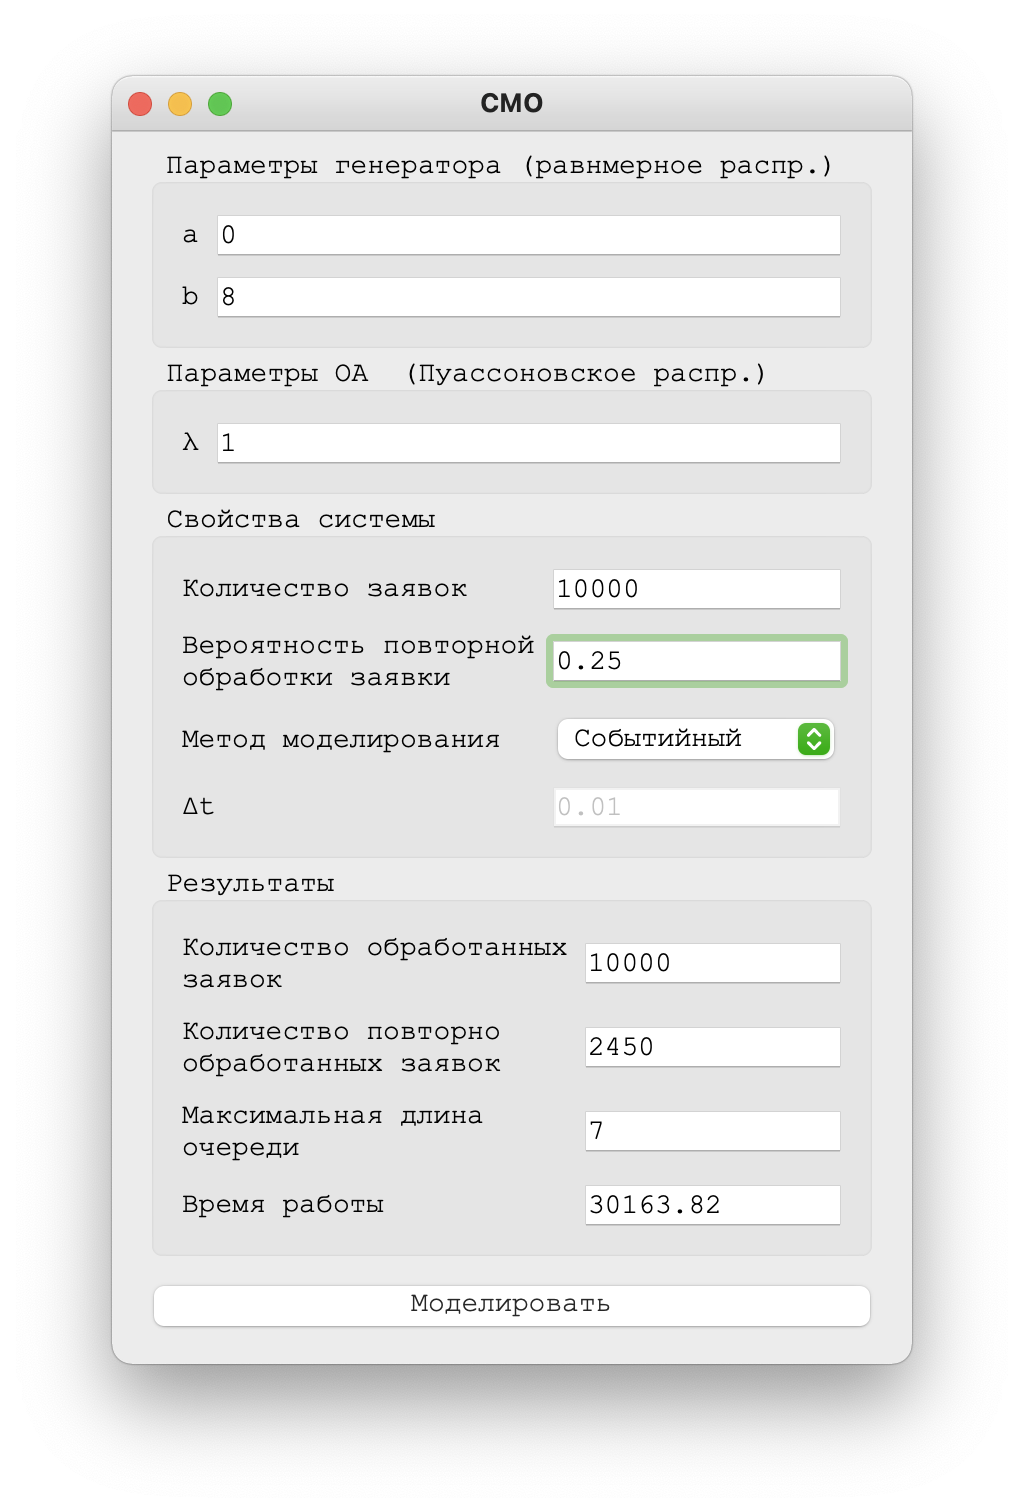
\includegraphics[width=1\linewidth]{1-25-s}
    \end{minipage}\hfill
    \begin{minipage}{0.55\textwidth}
      \centering
      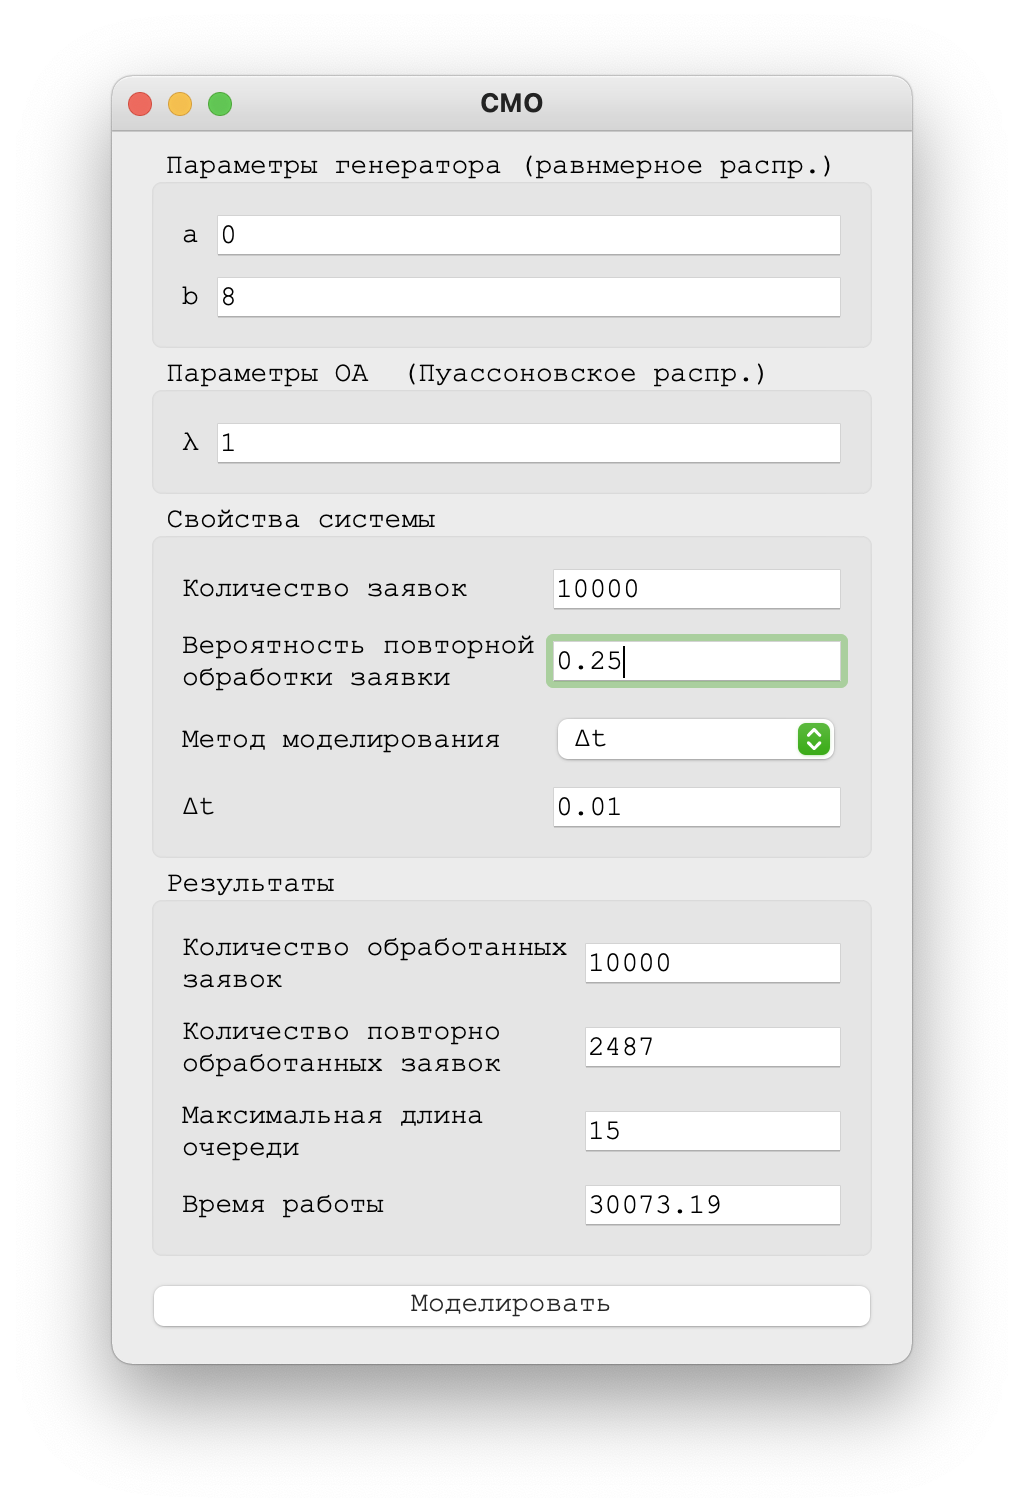
\includegraphics[width=1\linewidth]{1-25-t}
    \end{minipage}
    \caption{Пример работы программы при $p$ = 0.25 , $\lambda = 1$}
 \end{figure}


 \begin{figure}[!htb]
    \begin{minipage}{0.55\textwidth}
      \centering
      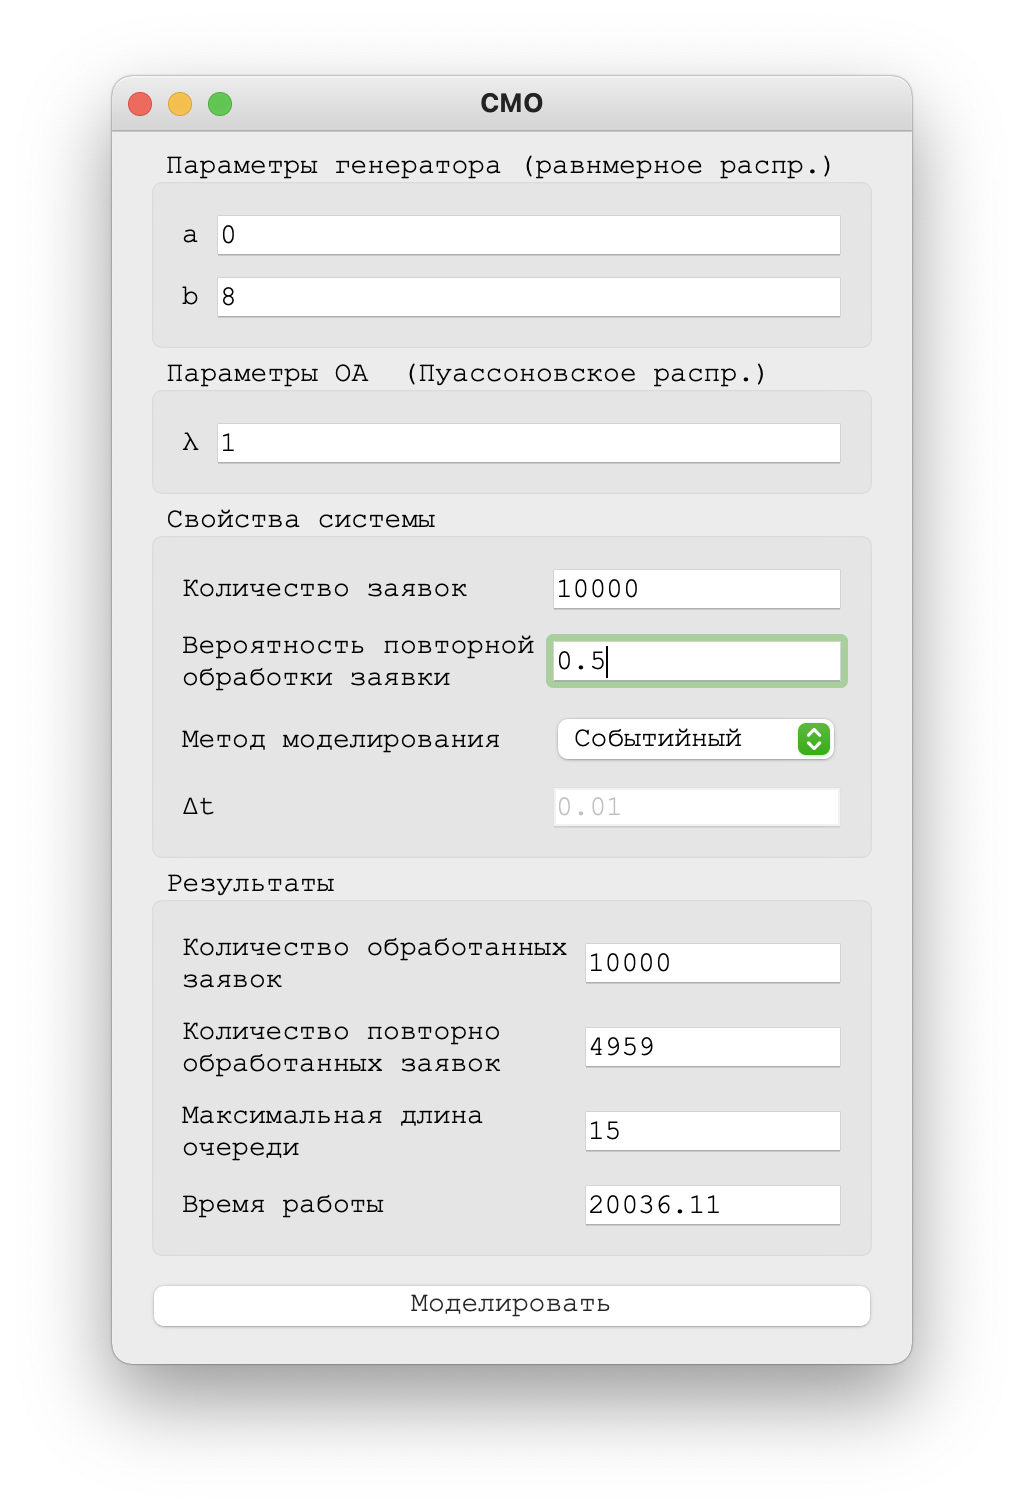
\includegraphics[width=1\linewidth]{1-5-s}
    \end{minipage}\hfill
    \begin{minipage}{0.55\textwidth}
      \centering
      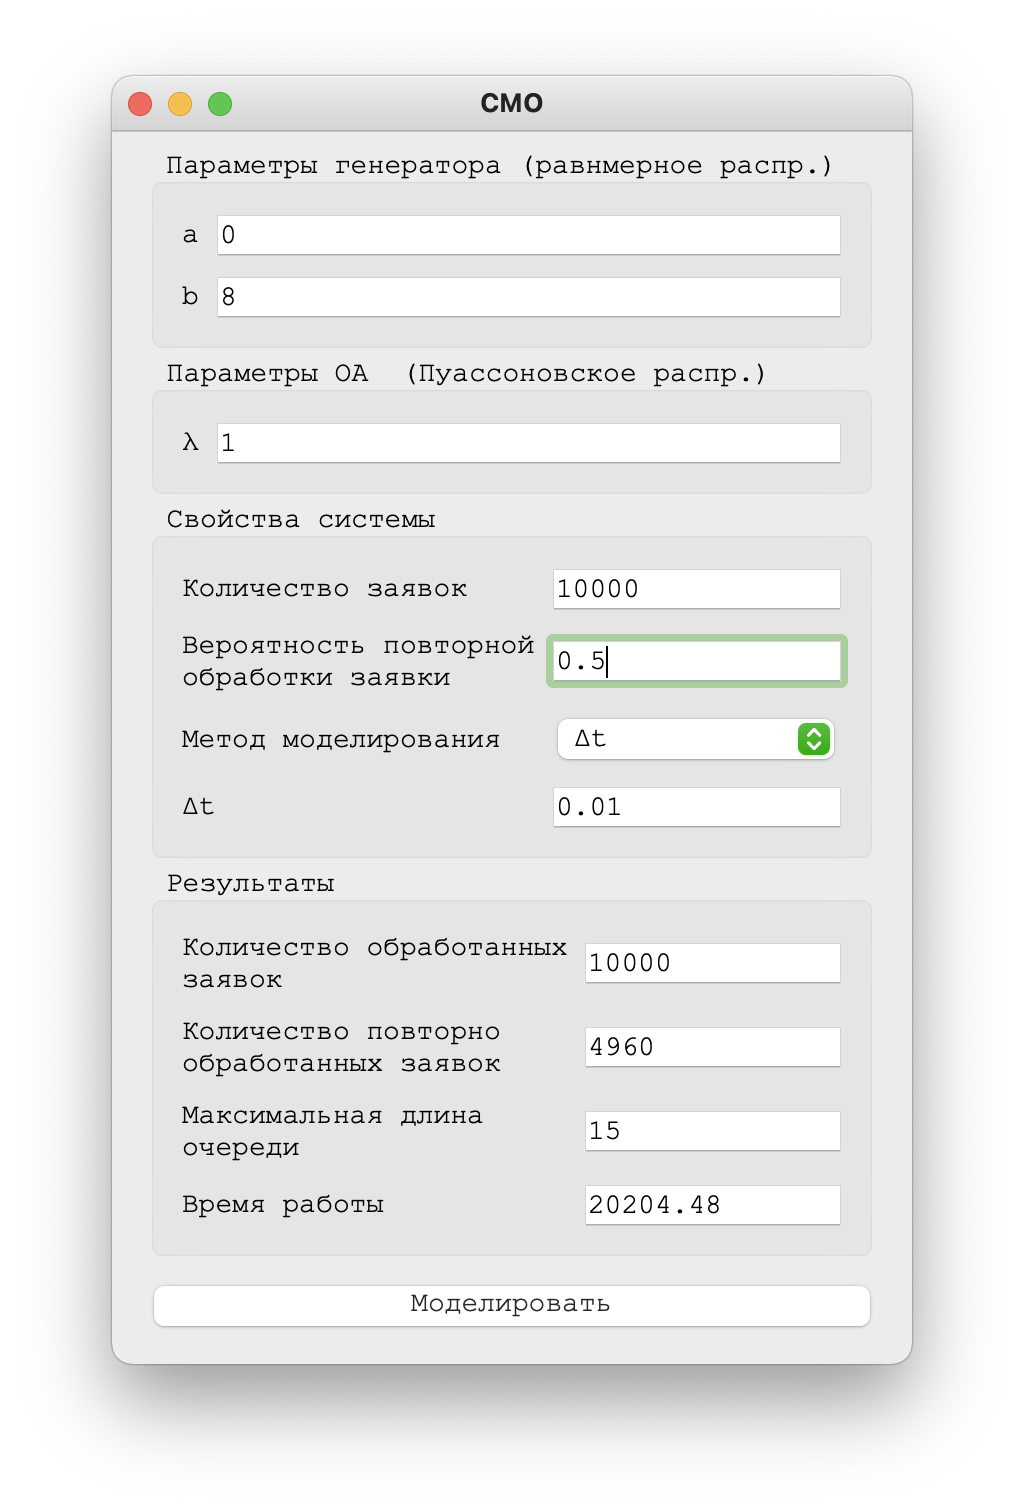
\includegraphics[width=1\linewidth]{1-5-t}
    \end{minipage}
    \caption{Пример работы программы при $p$ = 0.5 , $\lambda = 1$}
 \end{figure}

 
 \begin{figure}[!htb]
    \begin{minipage}{0.55\textwidth}
      \centering
      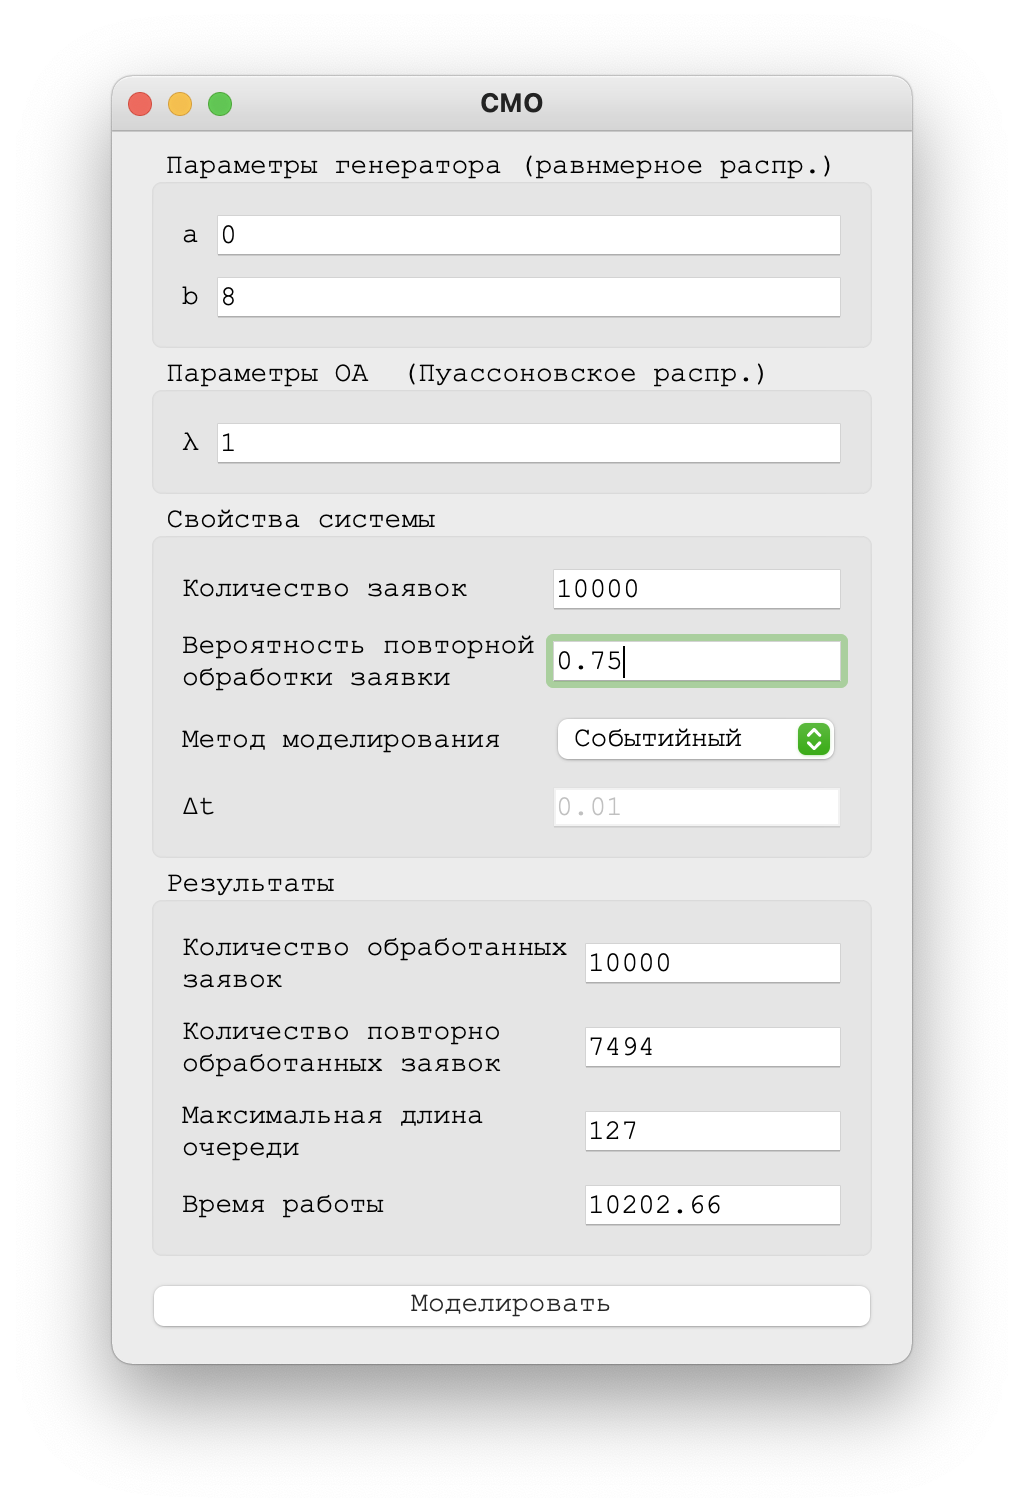
\includegraphics[width=1\linewidth]{1-75-s}
    \end{minipage}\hfill
    \begin{minipage}{0.55\textwidth}
      \centering
      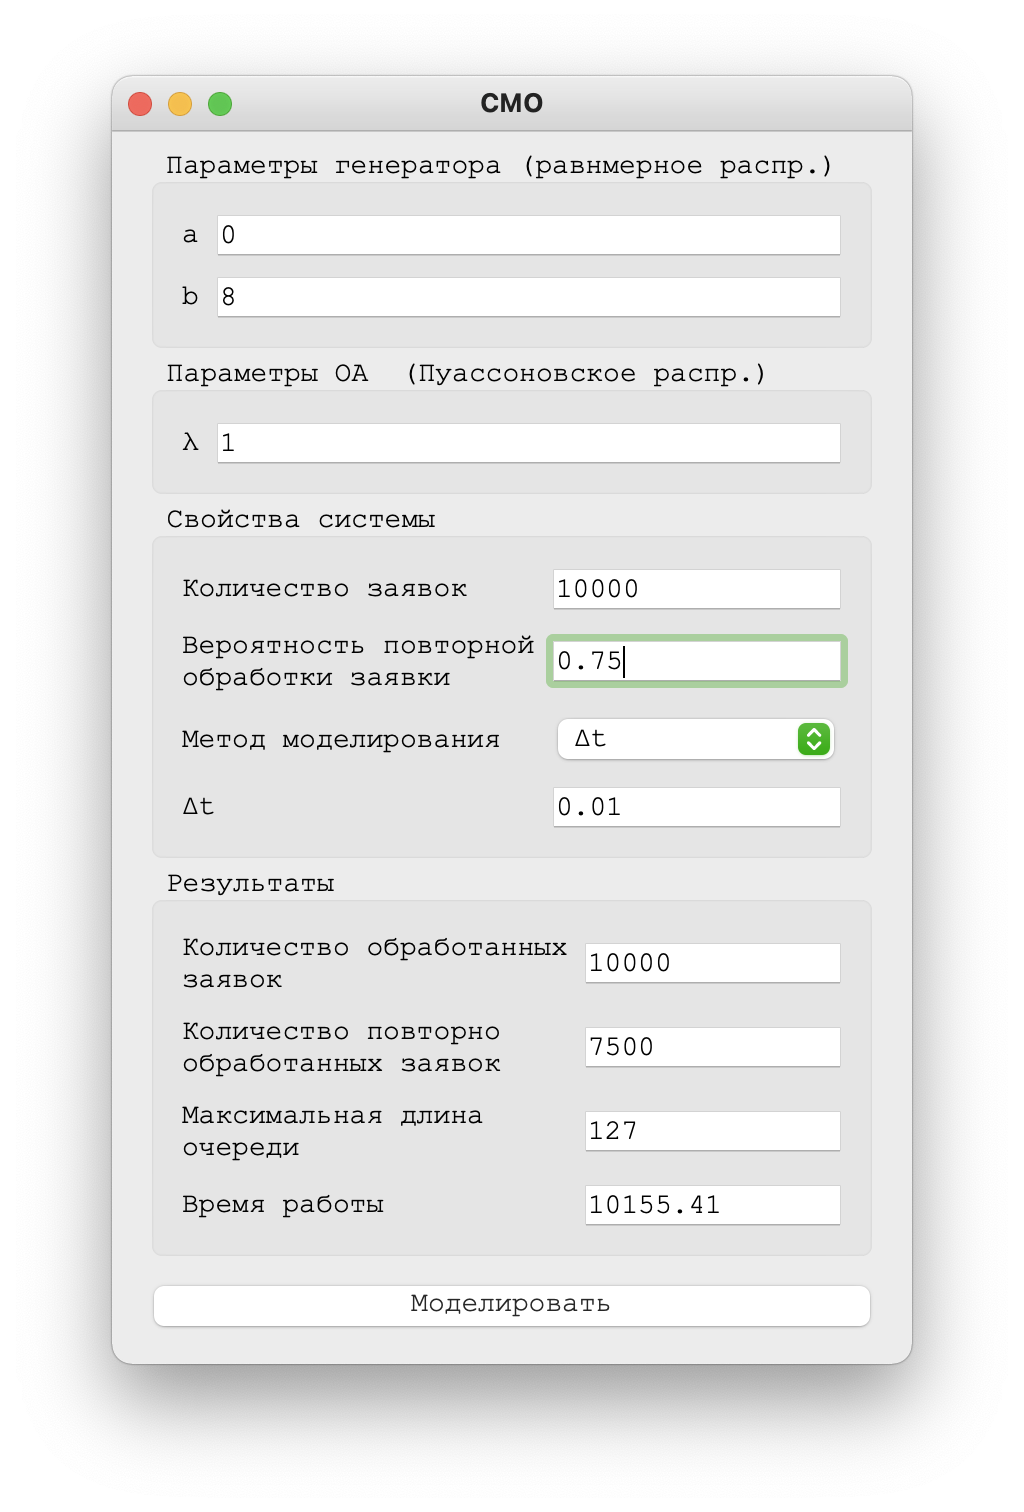
\includegraphics[width=1\linewidth]{1-75-t}
    \end{minipage}
    \caption{Пример работы программы при $p$ = 0.75 , $\lambda = 1$}
 \end{figure}


 \begin{figure}[!htb]
    \begin{minipage}{0.55\textwidth}
      \centering
      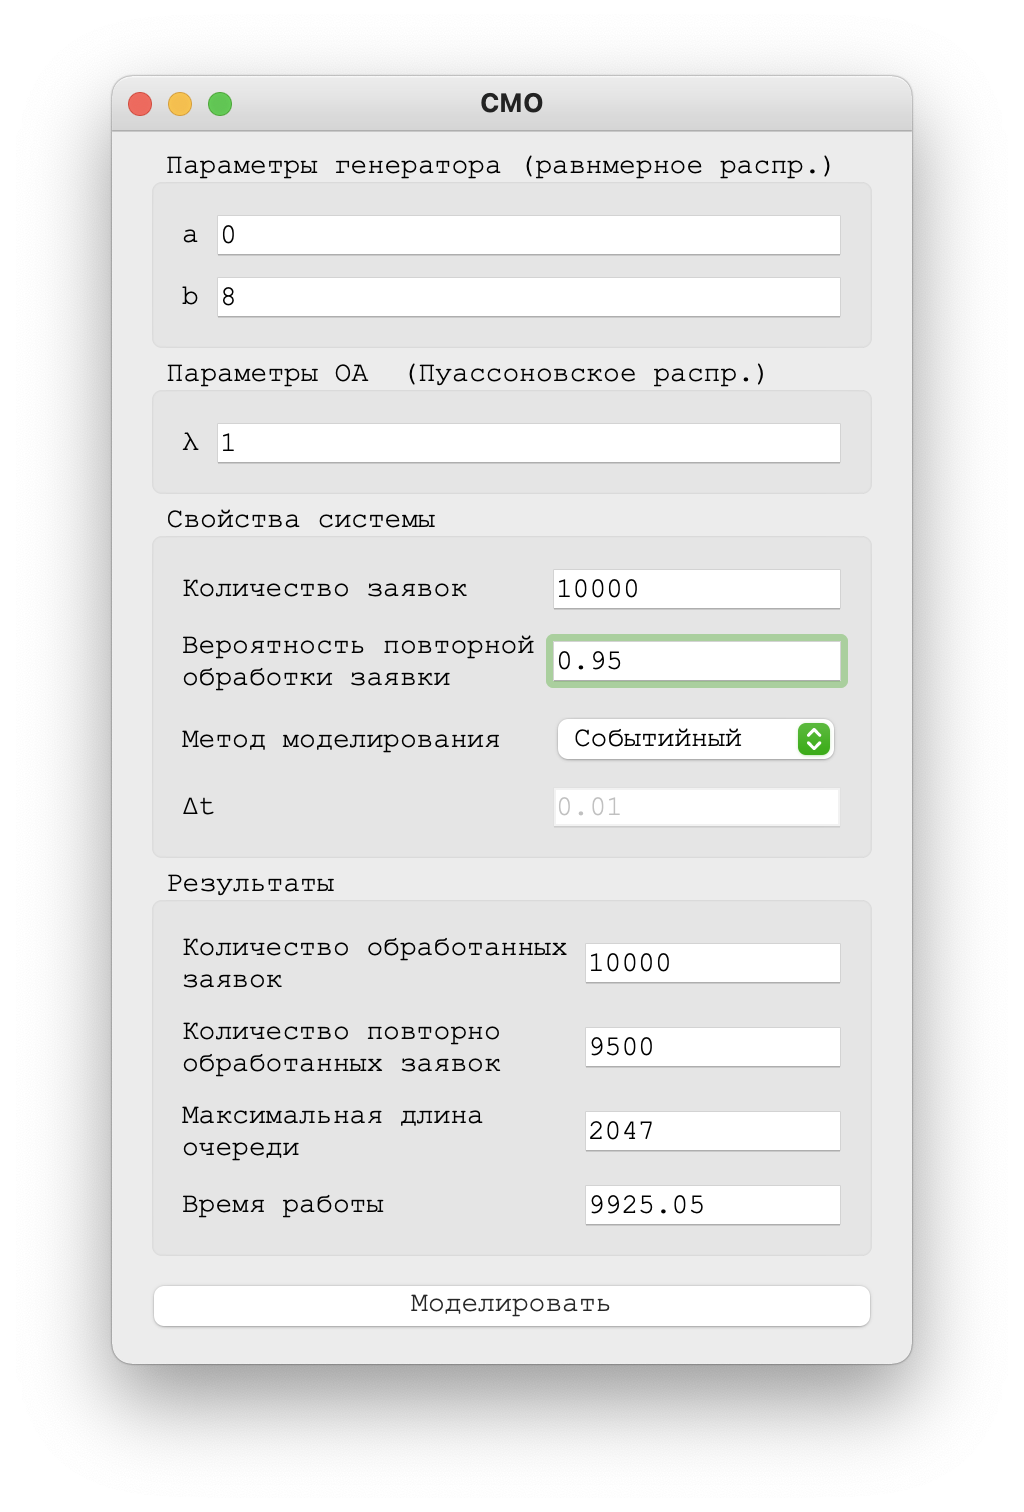
\includegraphics[width=1\linewidth]{1-95-s}
    \end{minipage}\hfill
    \begin{minipage}{0.55\textwidth}
      \centering
      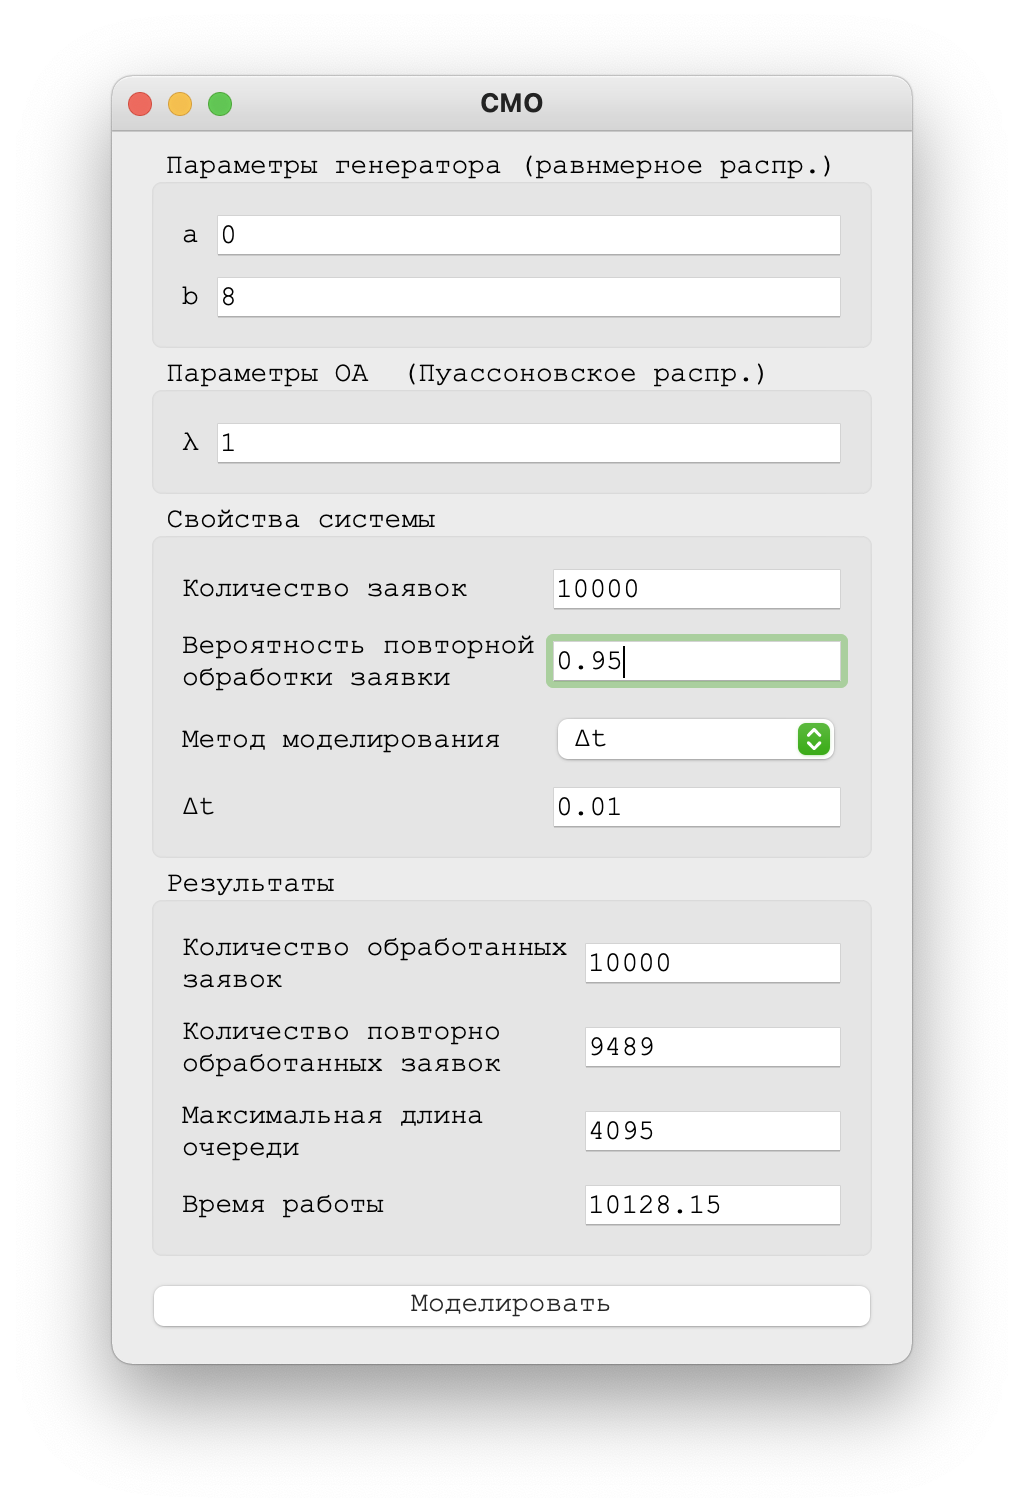
\includegraphics[width=1\linewidth]{1-95-t}
    \end{minipage}
    \caption{Пример работы программы при $p$ = 0.95 , $\lambda = 1$}
 \end{figure}


 \begin{figure}[!htb]
    \begin{minipage}{0.55\textwidth}
      \centering
      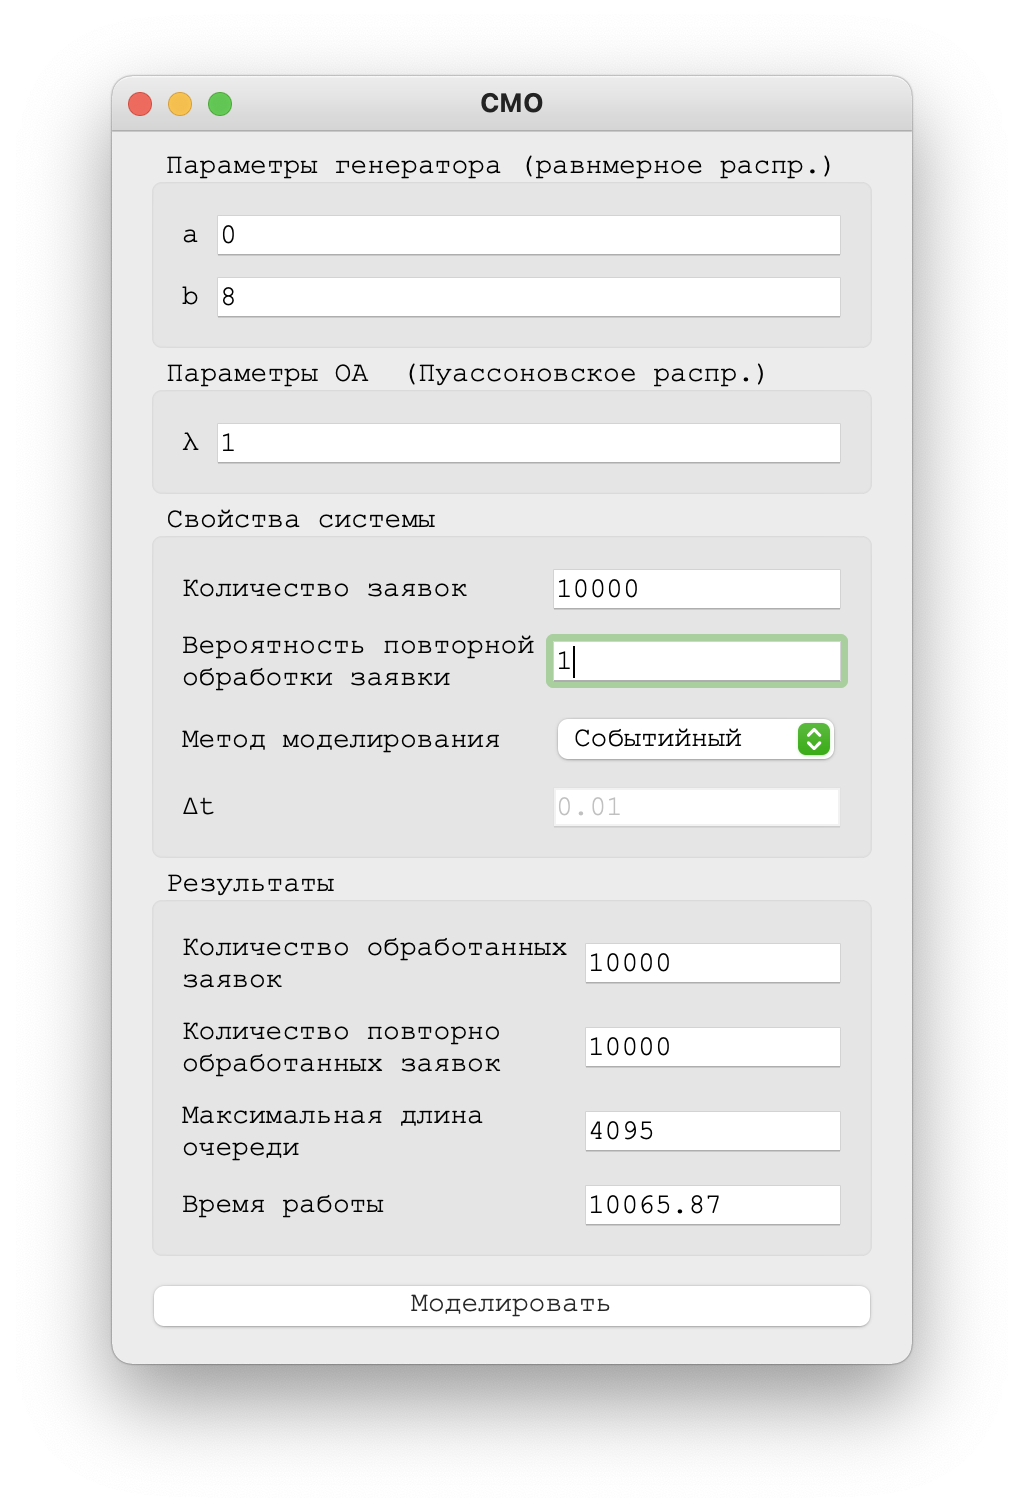
\includegraphics[width=1\linewidth]{1-1-s}
    \end{minipage}\hfill
    \begin{minipage}{0.55\textwidth}
      \centering
      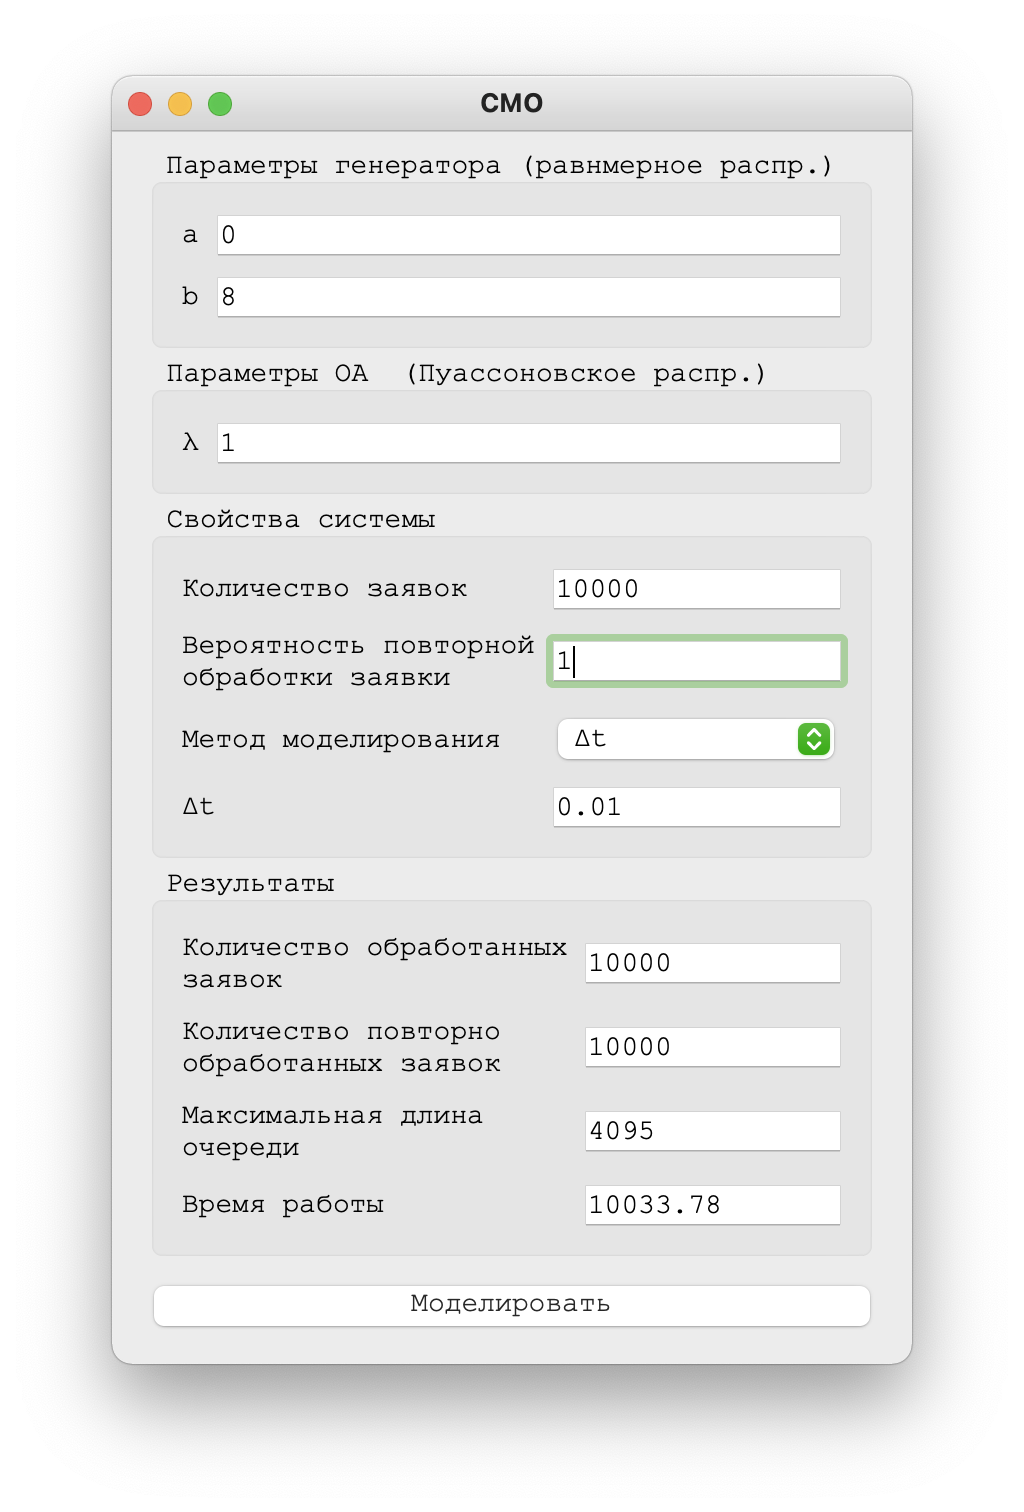
\includegraphics[width=1\linewidth]{1-1-t}
    \end{minipage}
    \caption{Пример работы программы при $p$ = 1 , $\lambda = 1$}
 \end{figure}



 \begin{figure}[!htb]
    \begin{minipage}{0.55\textwidth}
      \centering
      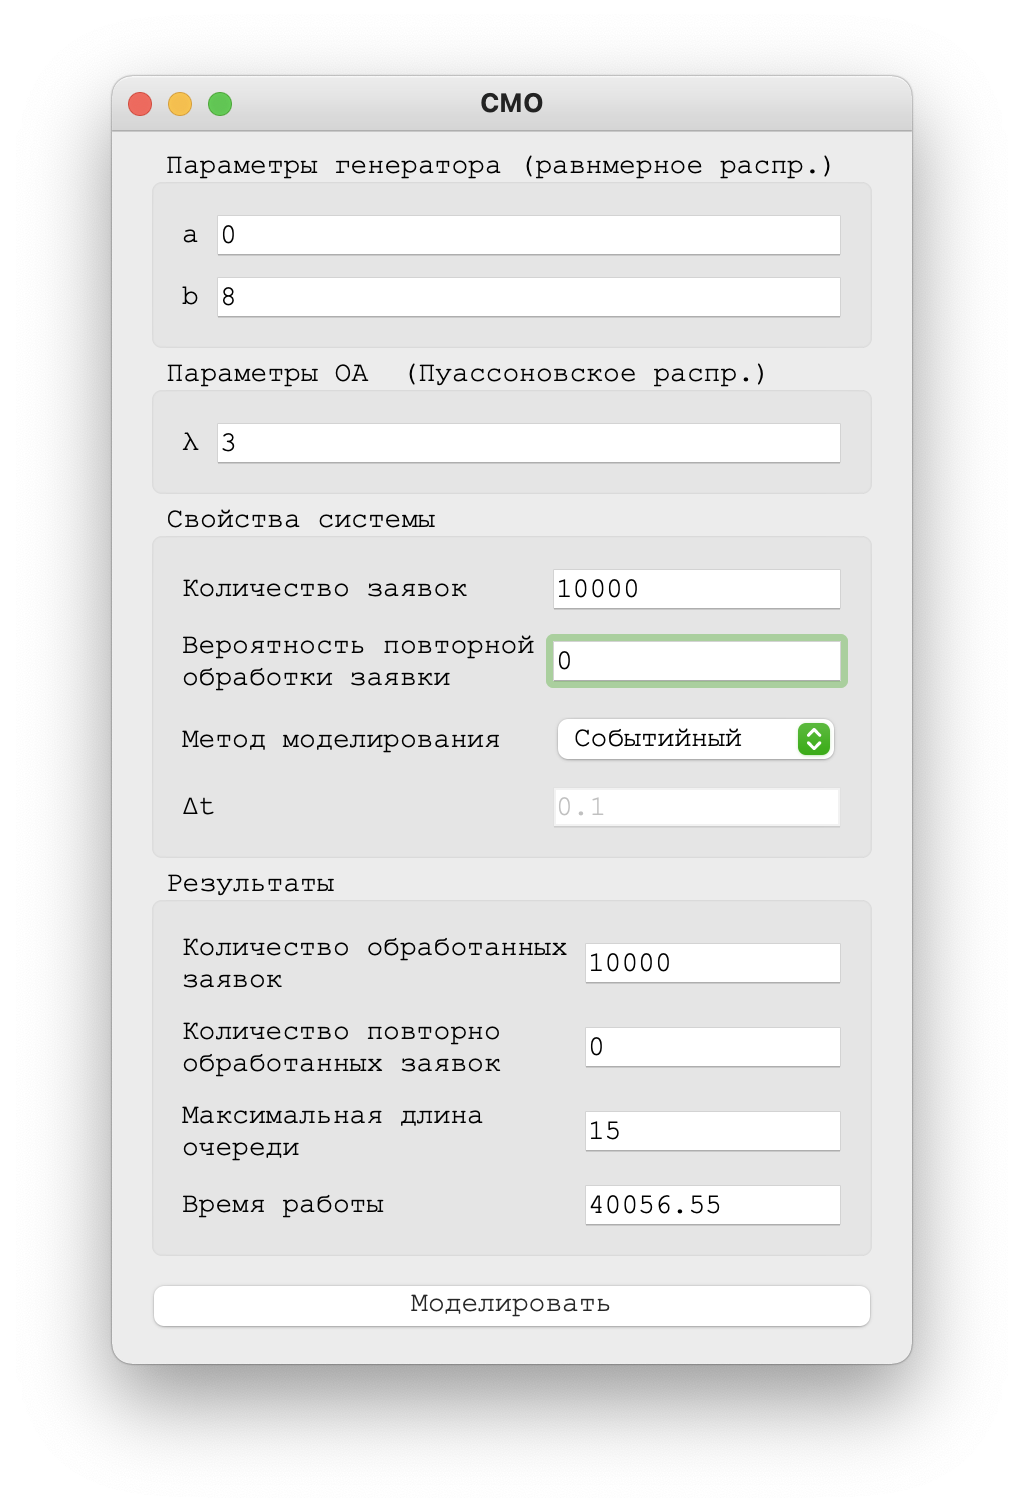
\includegraphics[width=1\linewidth]{3-0-s}
    \end{minipage}\hfill
    \begin{minipage}{0.55\textwidth}
      \centering
      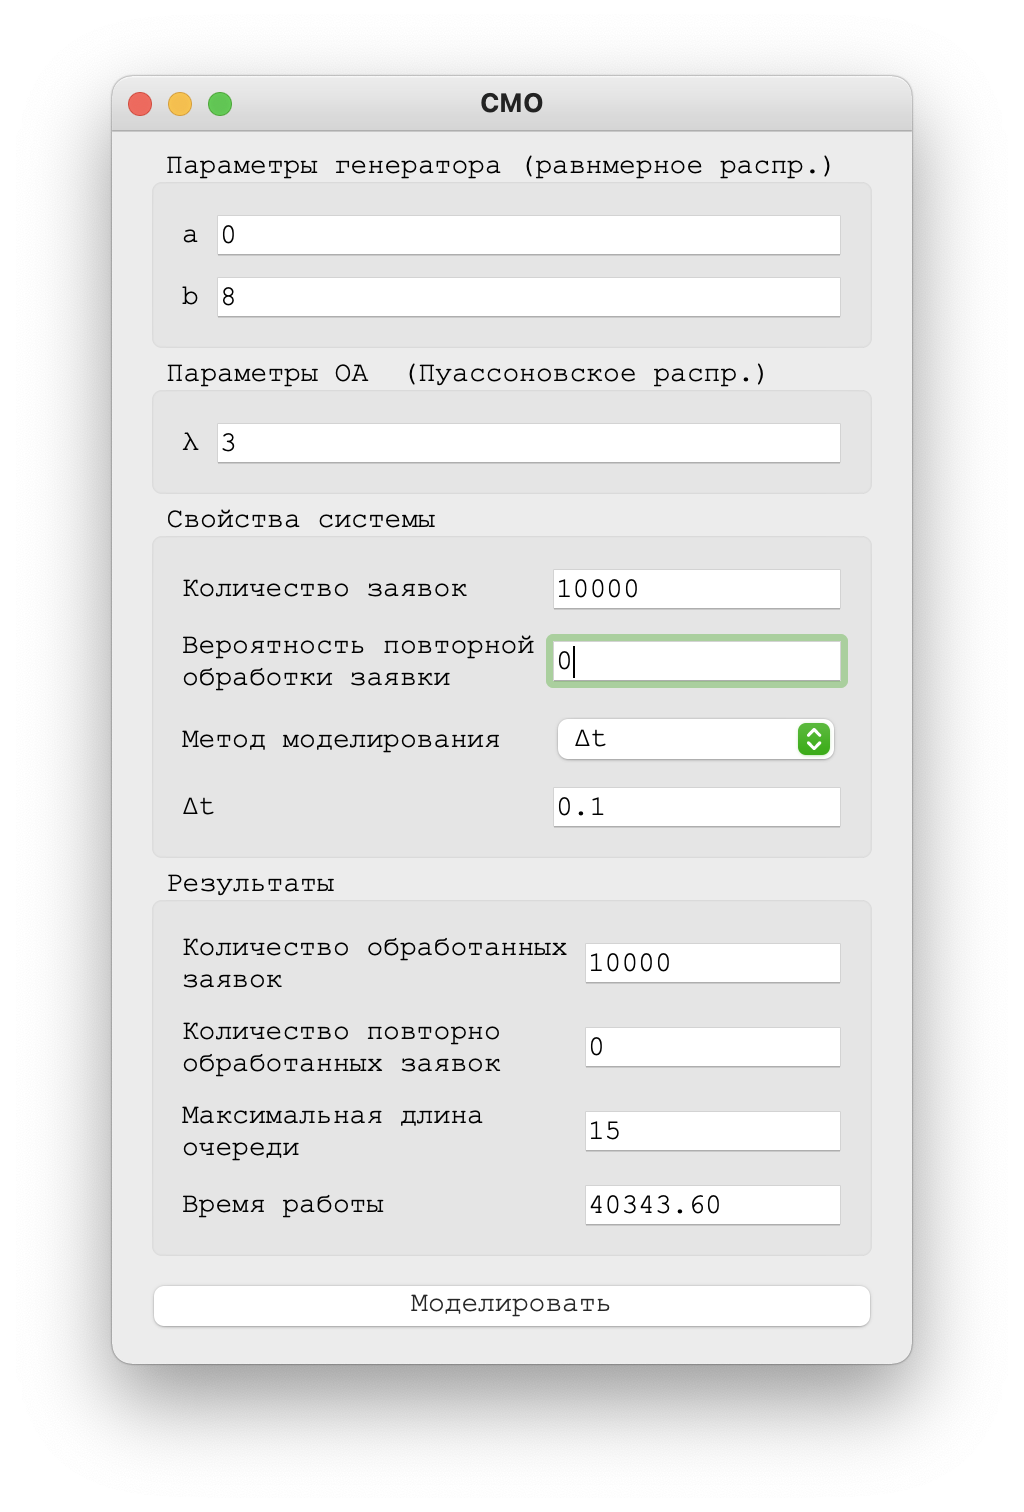
\includegraphics[width=1\linewidth]{3-0-t}
    \end{minipage}
    \caption{Пример работы программы при $p$ = 0 , $\lambda = 3$}
 \end{figure}
 


 \begin{figure}[!htb]
    \begin{minipage}{0.55\textwidth}
      \centering
      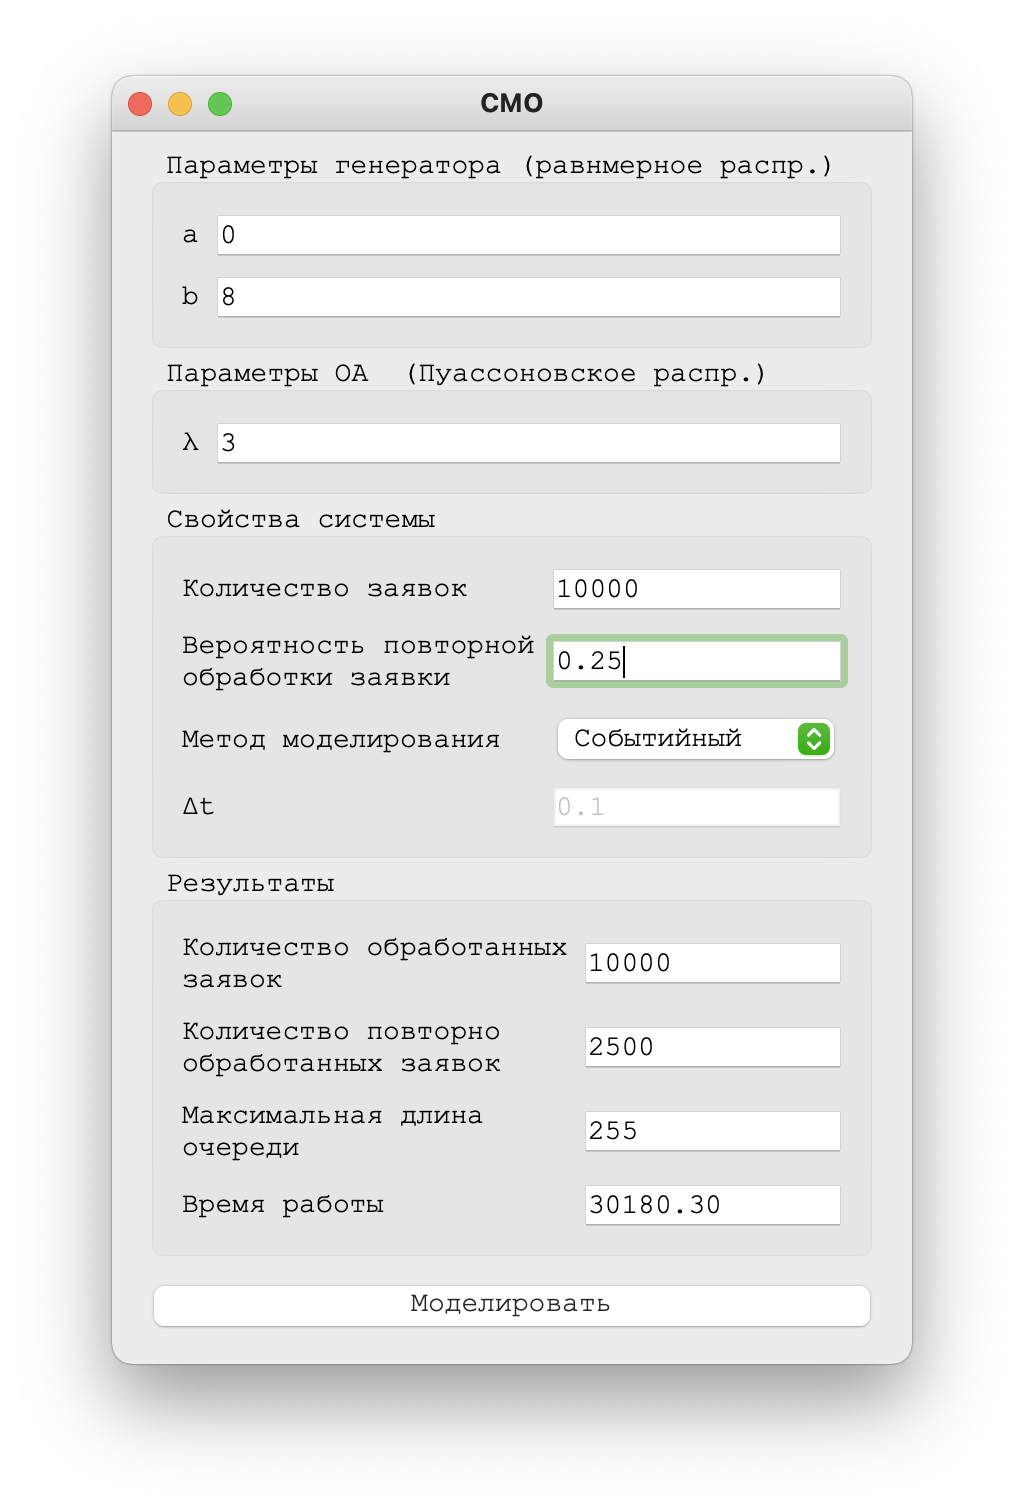
\includegraphics[width=1\linewidth]{3-25-s}
    \end{minipage}\hfill
    \begin{minipage}{0.55\textwidth}
      \centering
      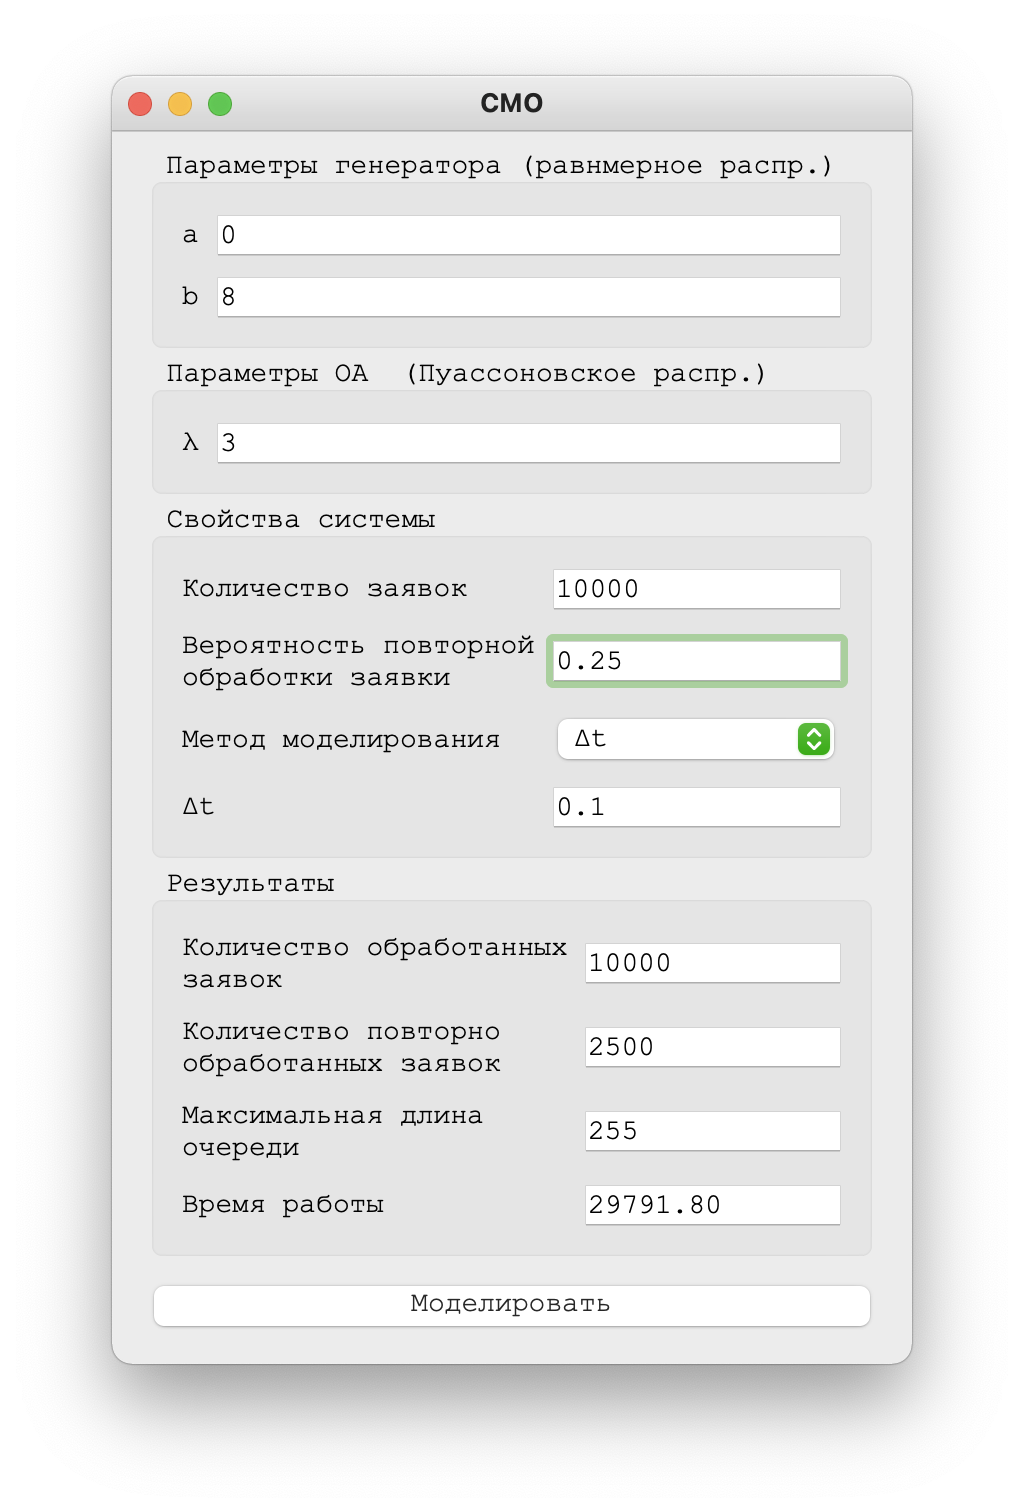
\includegraphics[width=1\linewidth]{3-25-t}
    \end{minipage}
    \caption{Пример работы программы при $p$ = 0.25 , $\lambda = 3$}
 \end{figure}


 \begin{figure}[!htb]
    \begin{minipage}{0.55\textwidth}
      \centering
      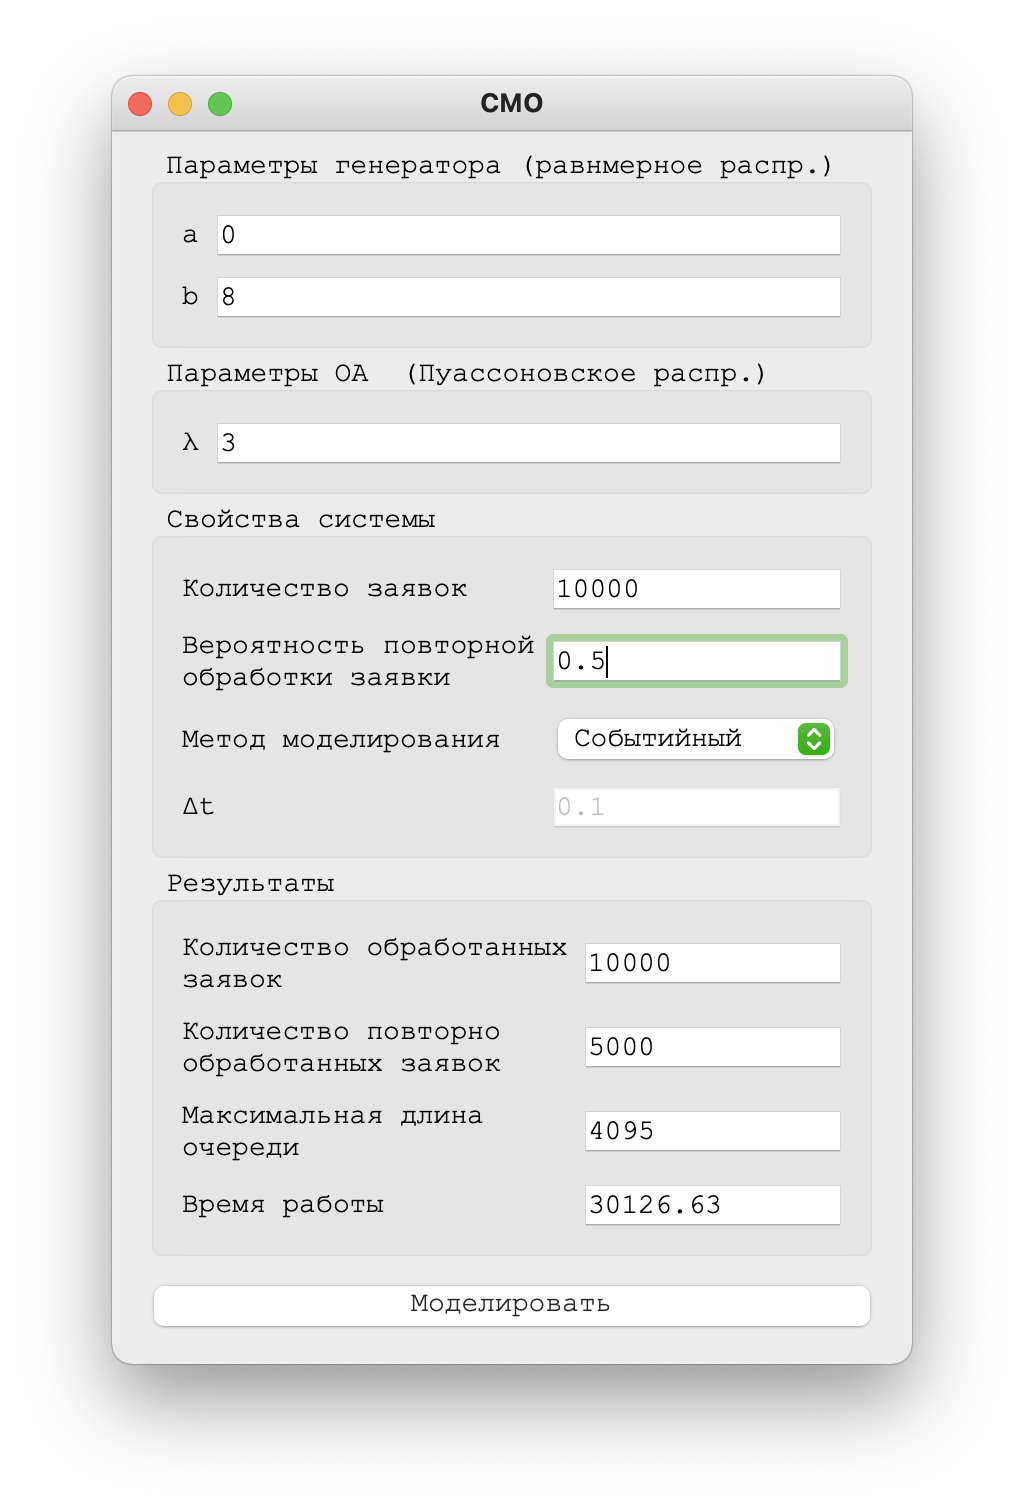
\includegraphics[width=1\linewidth]{3-50-s}
    \end{minipage}\hfill
    \begin{minipage}{0.55\textwidth}
      \centering
      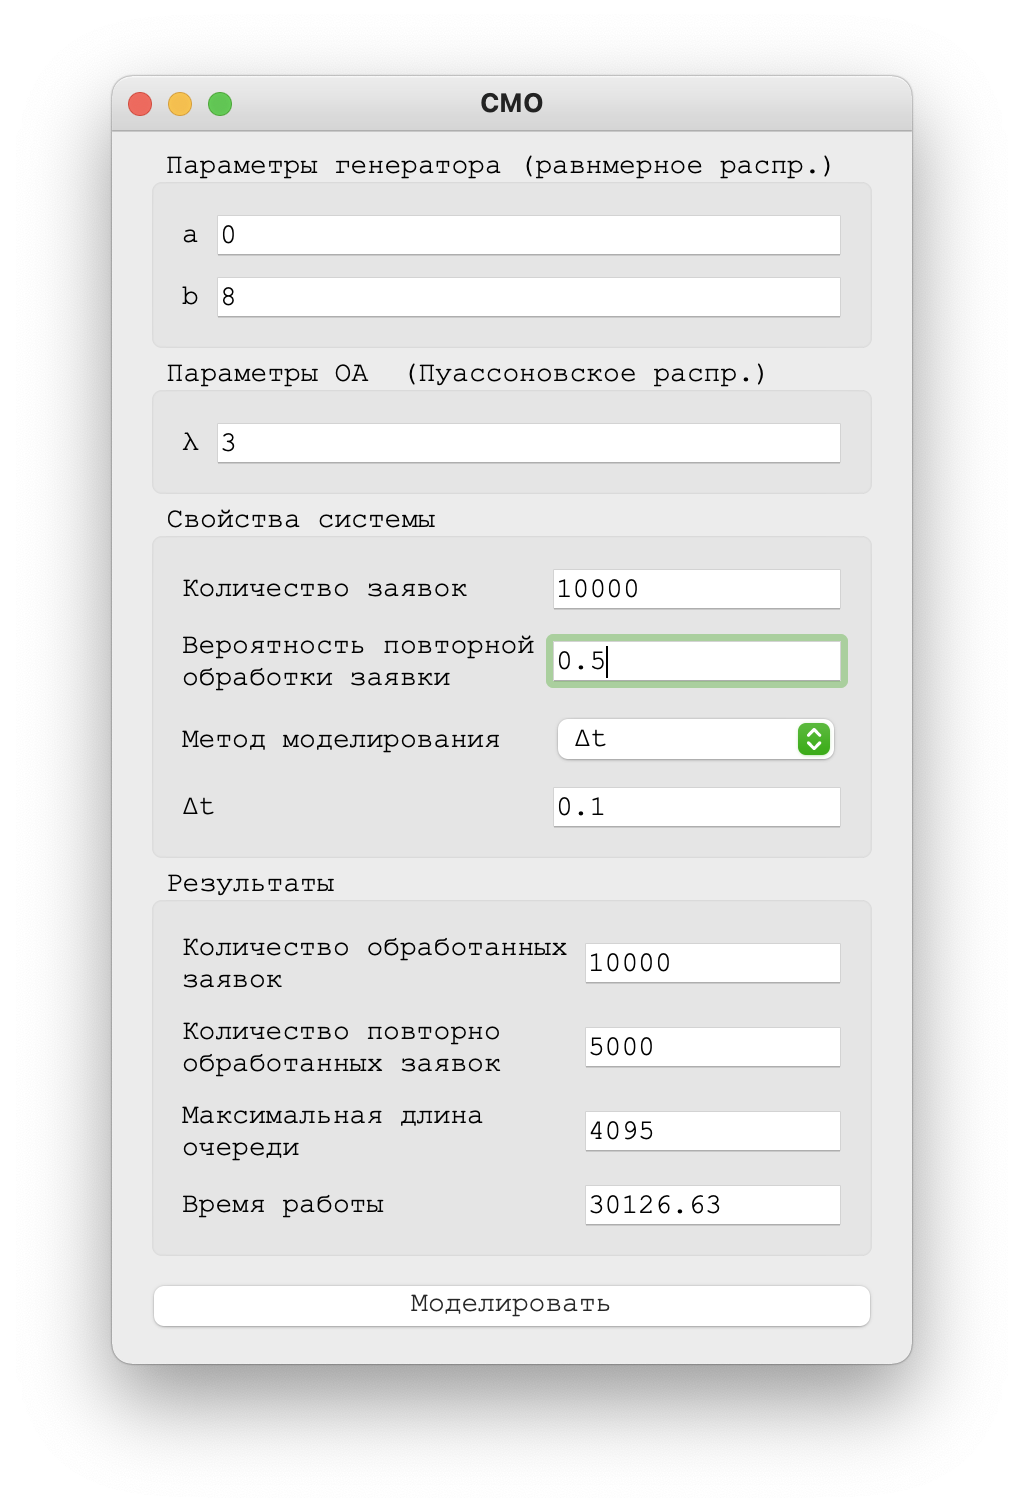
\includegraphics[width=1\linewidth]{3-50-t}
    \end{minipage}
    \caption{Пример работы программы при $p$ = 0.5 , $\lambda = 3$}
 \end{figure}

 
 \begin{figure}[!htb]
    \begin{minipage}{0.55\textwidth}
      \centering
      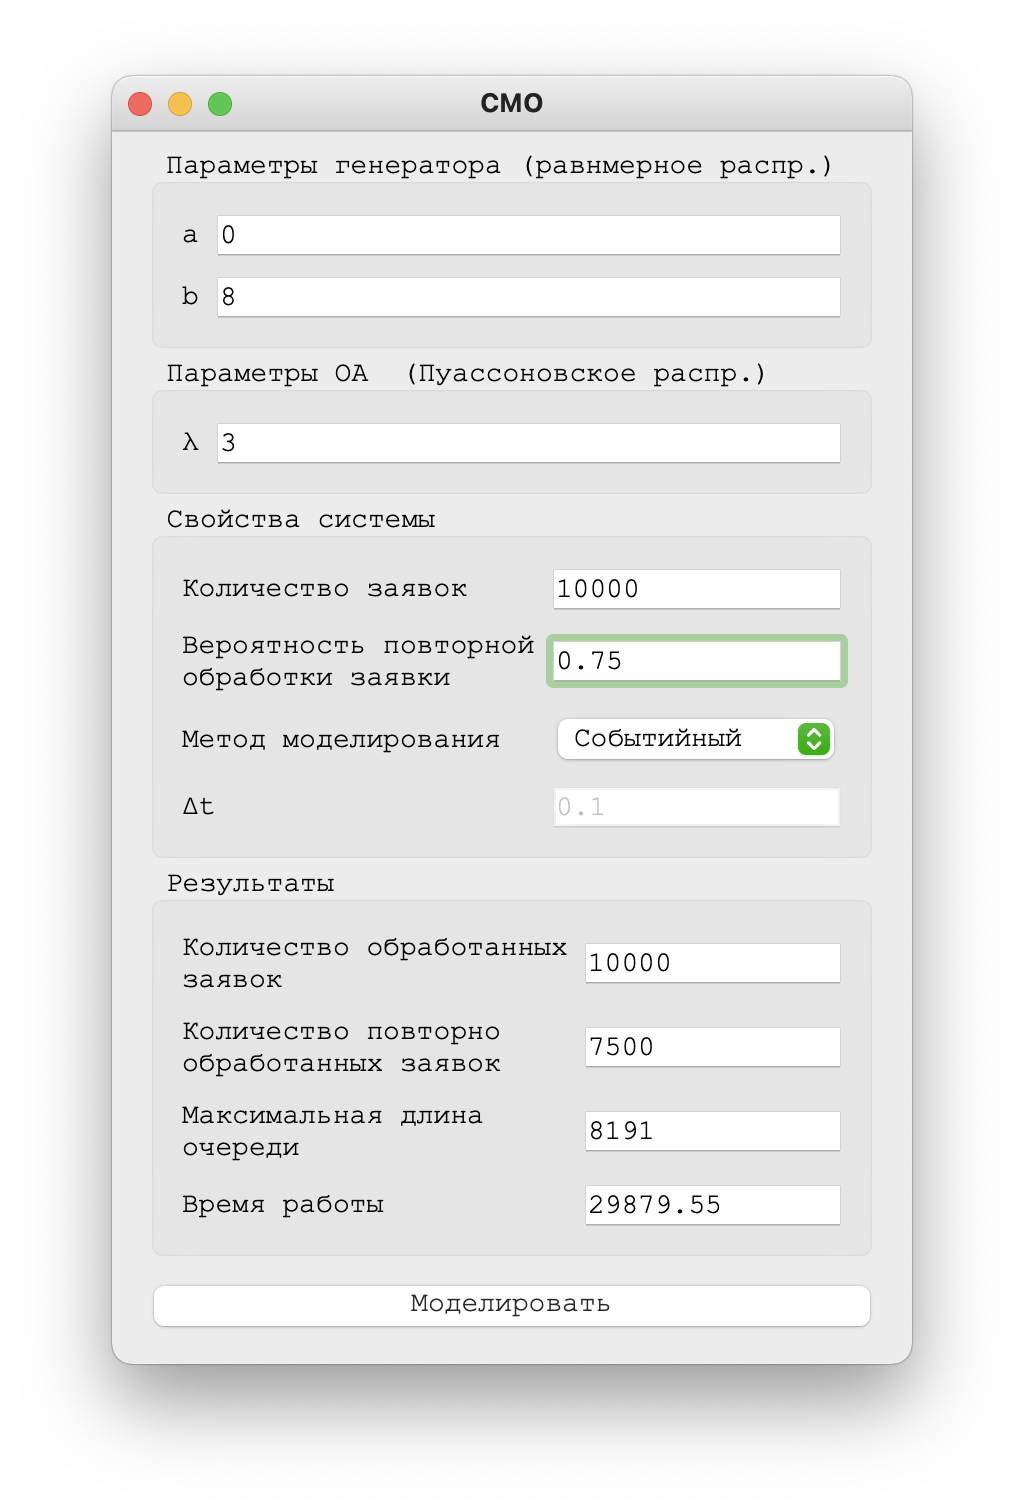
\includegraphics[width=1\linewidth]{3-75-s}
    \end{minipage}\hfill
    \begin{minipage}{0.55\textwidth}
      \centering
      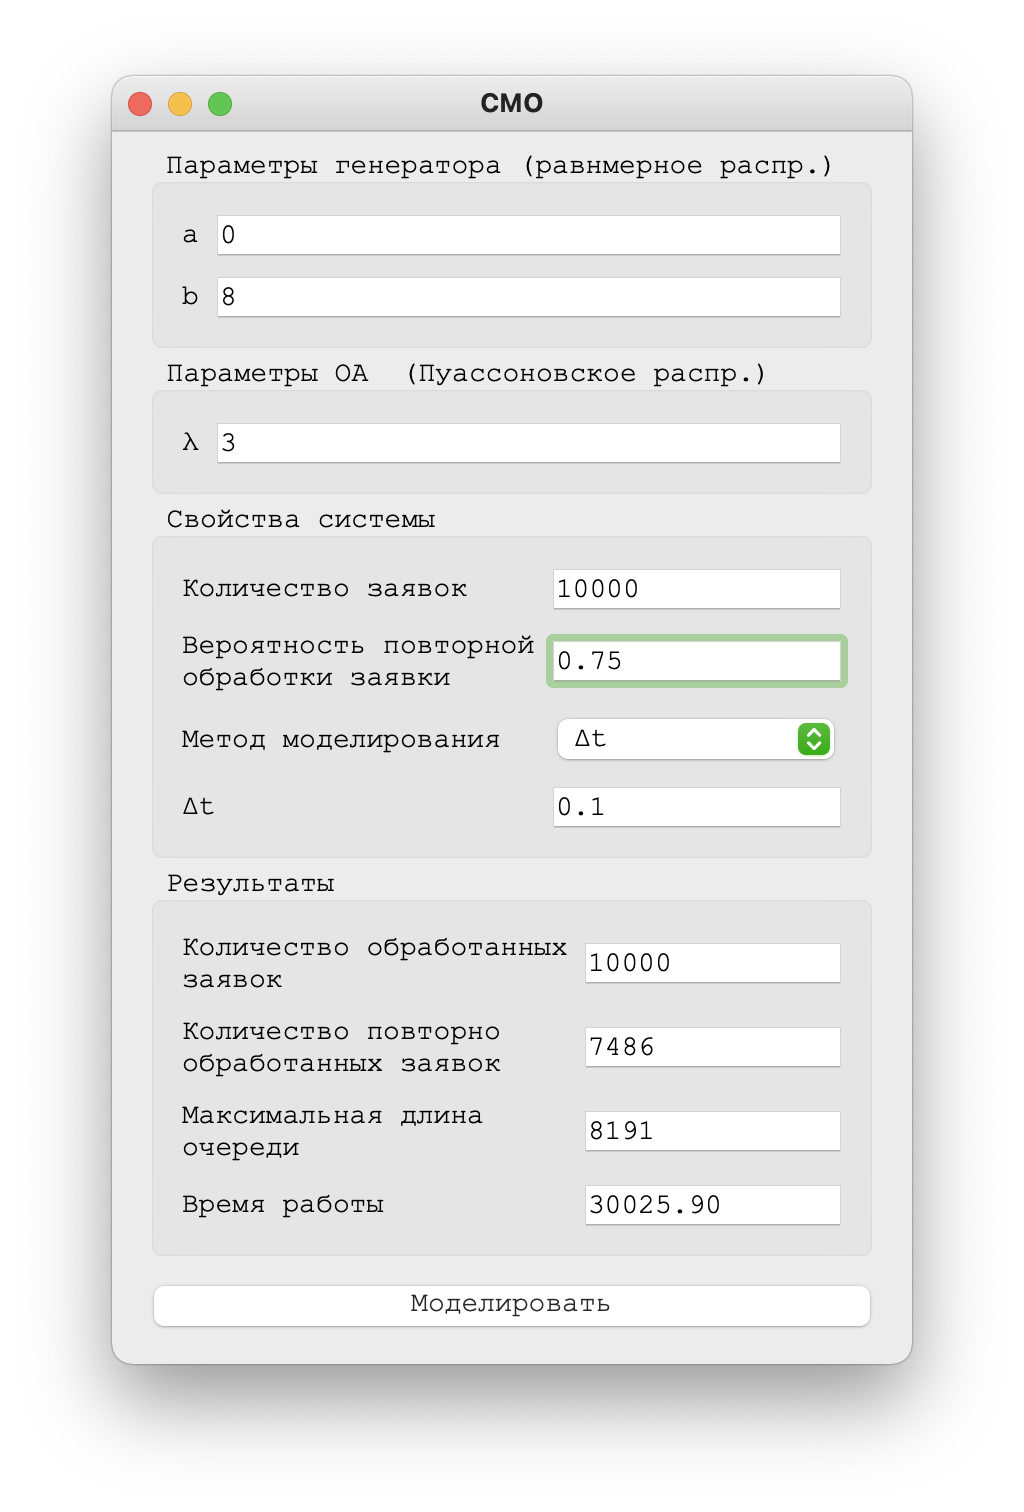
\includegraphics[width=1\linewidth]{3-75-t}
    \end{minipage}
    \caption{Пример работы программы при $p$ = 0.75 , $\lambda = 3$}
 \end{figure}


 \begin{figure}[!htb]
    \begin{minipage}{0.55\textwidth}
      \centering
      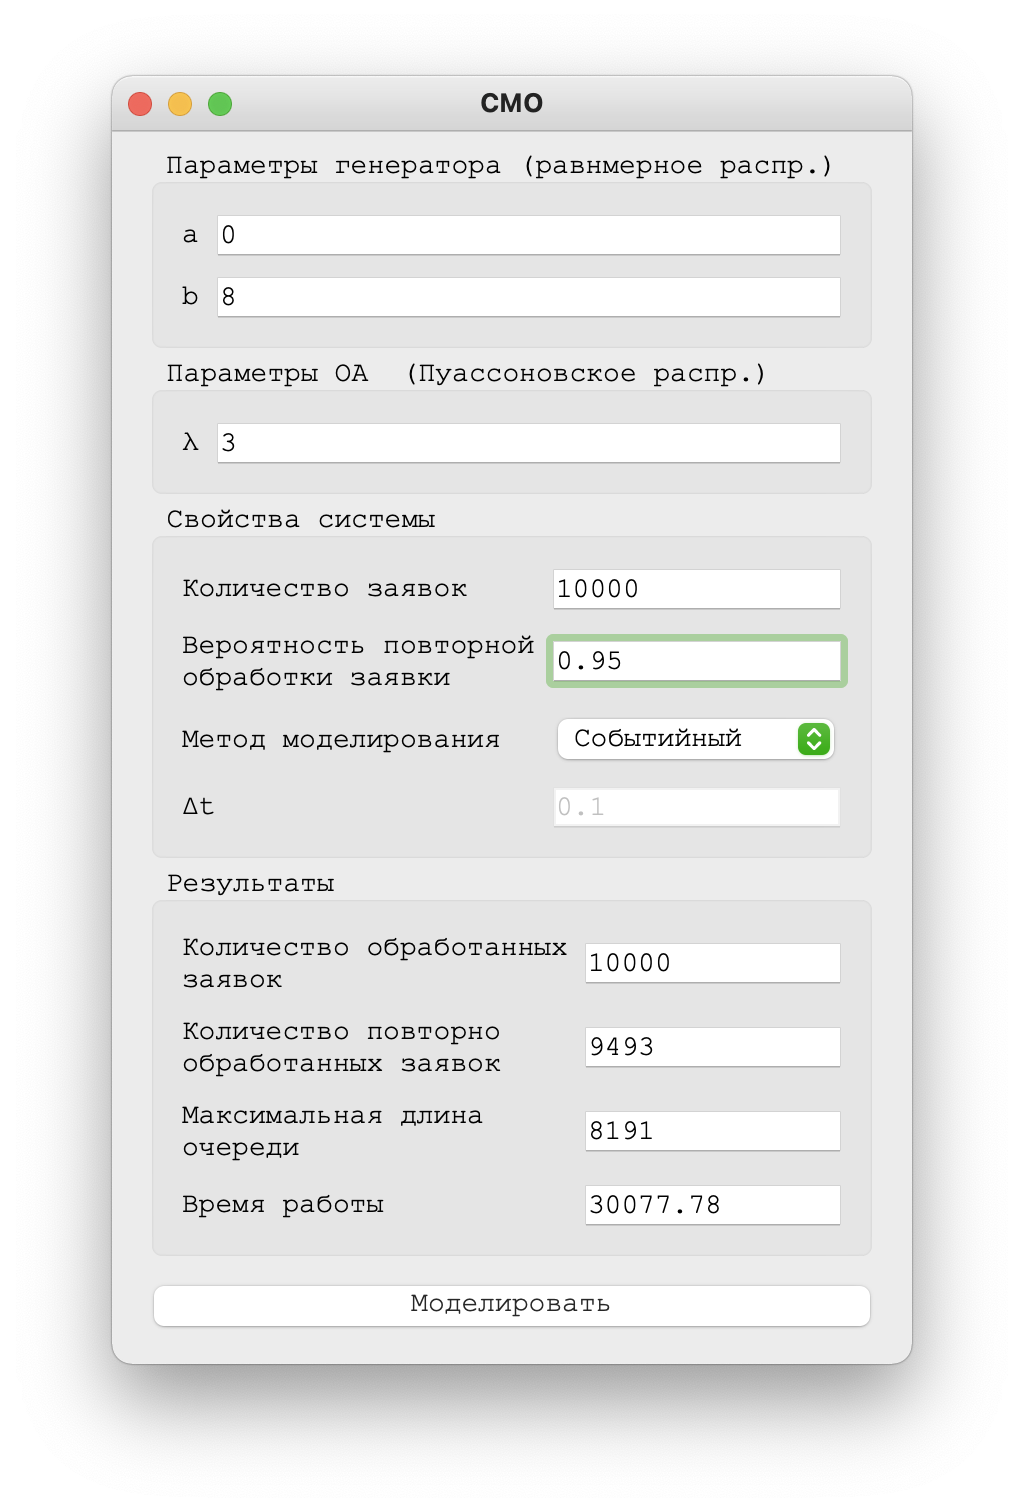
\includegraphics[width=1\linewidth]{3-95-s}
    \end{minipage}\hfill
    \begin{minipage}{0.55\textwidth}
      \centering
      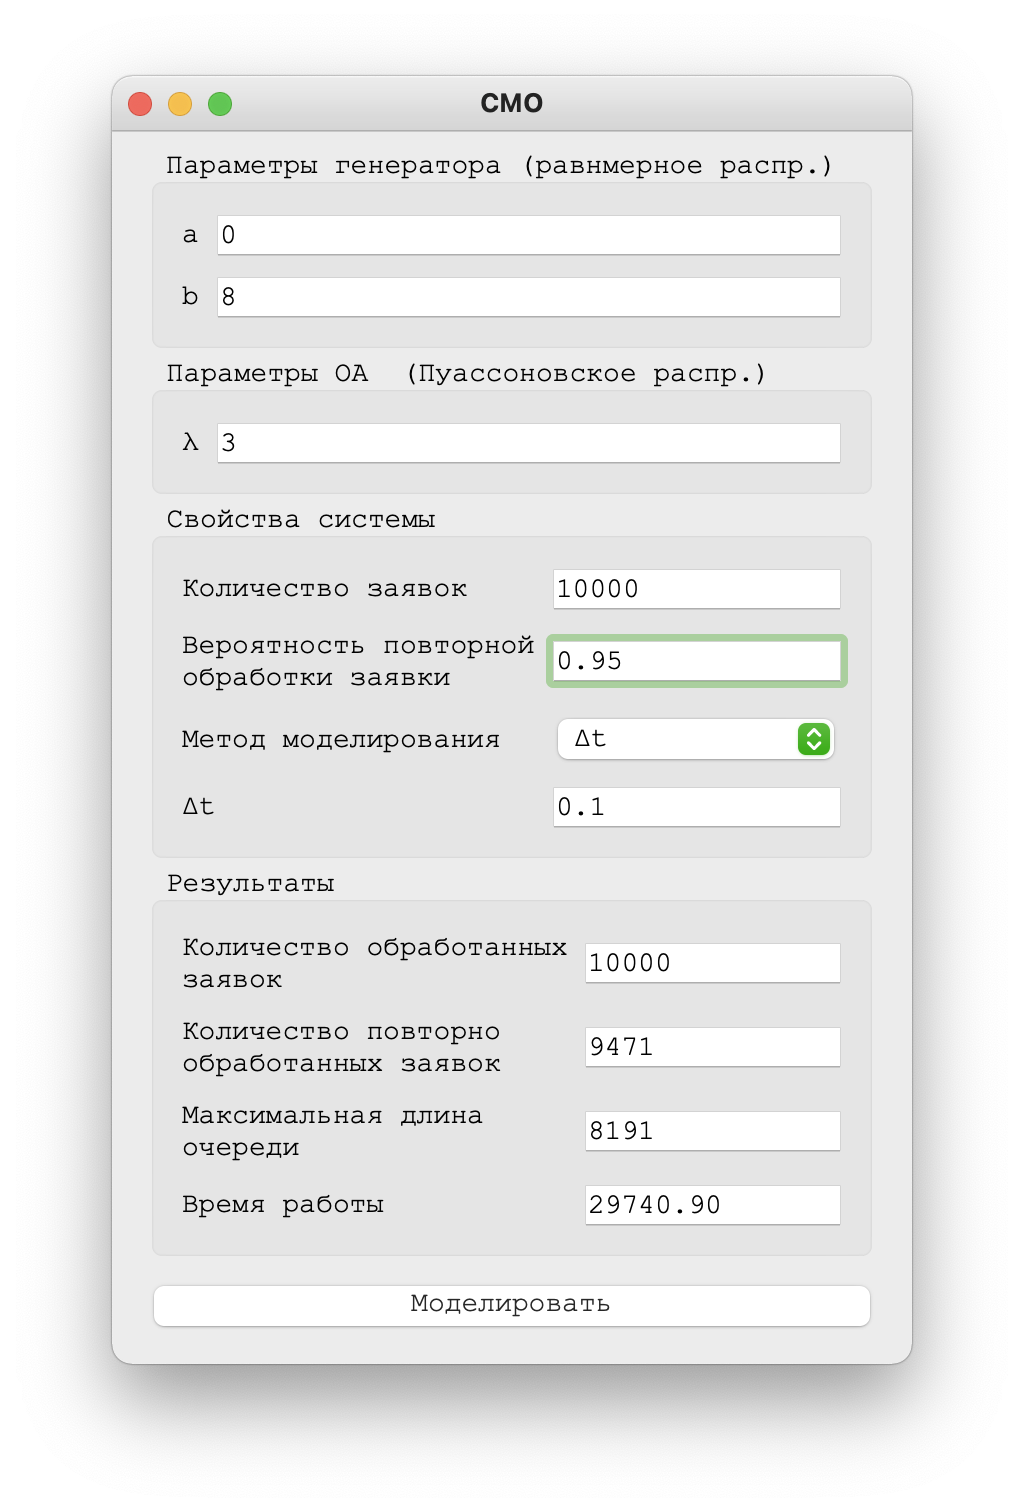
\includegraphics[width=1\linewidth]{3-95-t}
    \end{minipage}
    \caption{Пример работы программы при $p$ = 0.95 , $\lambda = 3$}
 \end{figure}


 \begin{figure}[!htb]
    \begin{minipage}{0.55\textwidth}
      \centering
      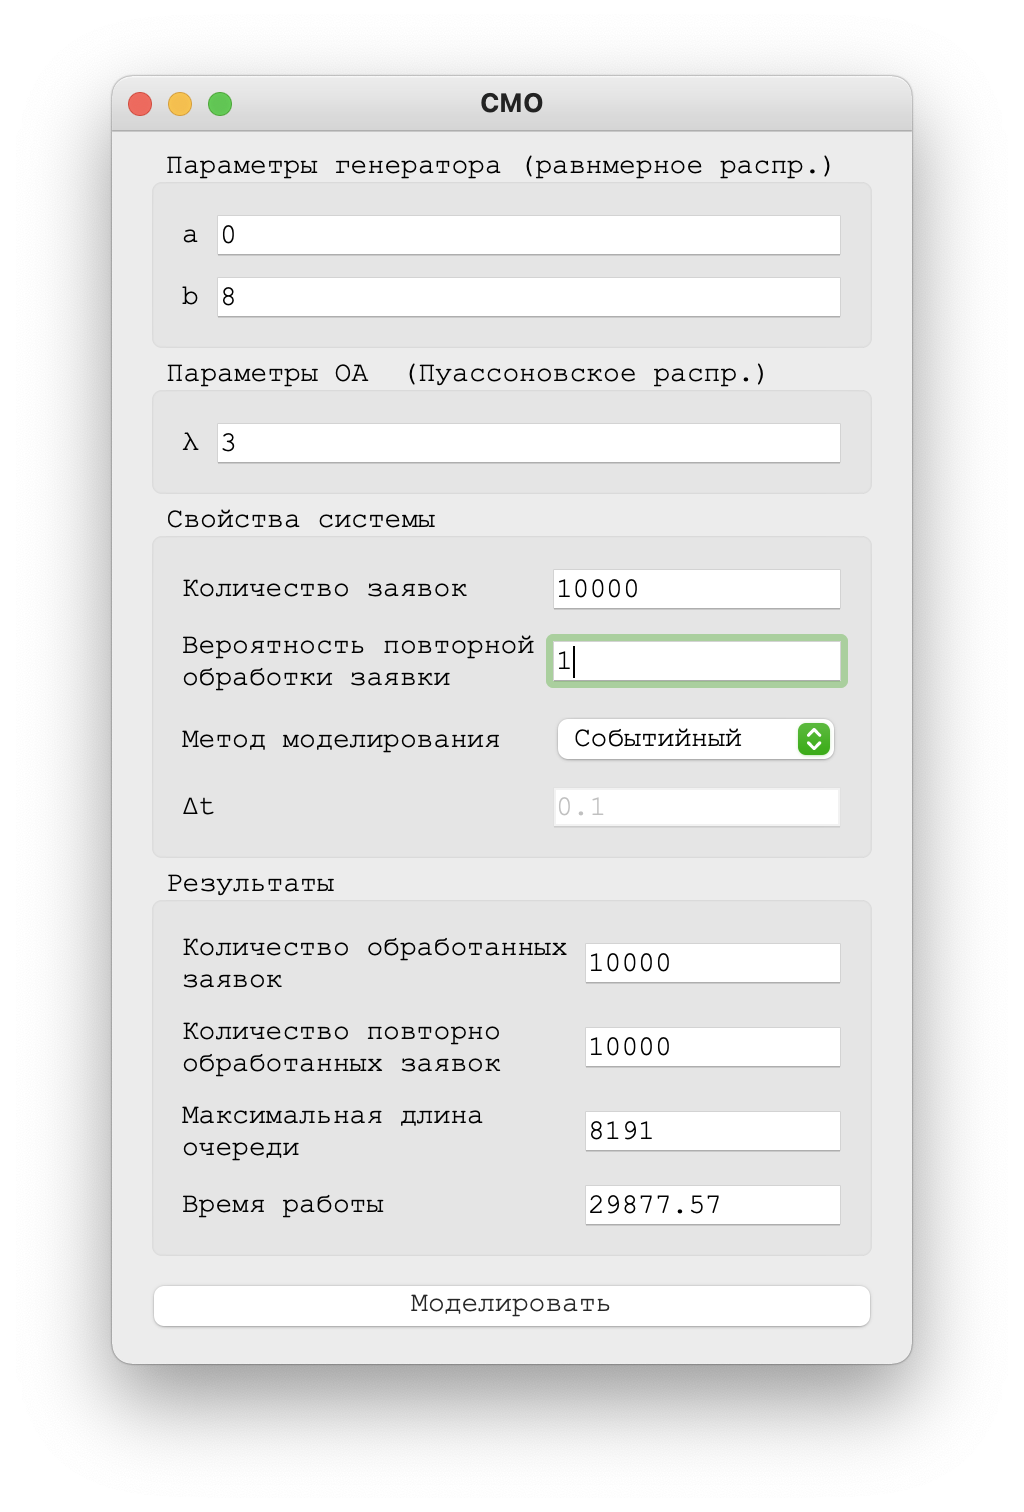
\includegraphics[width=1\linewidth]{3-1-s}
    \end{minipage}\hfill
    \begin{minipage}{0.55\textwidth}
      \centering
      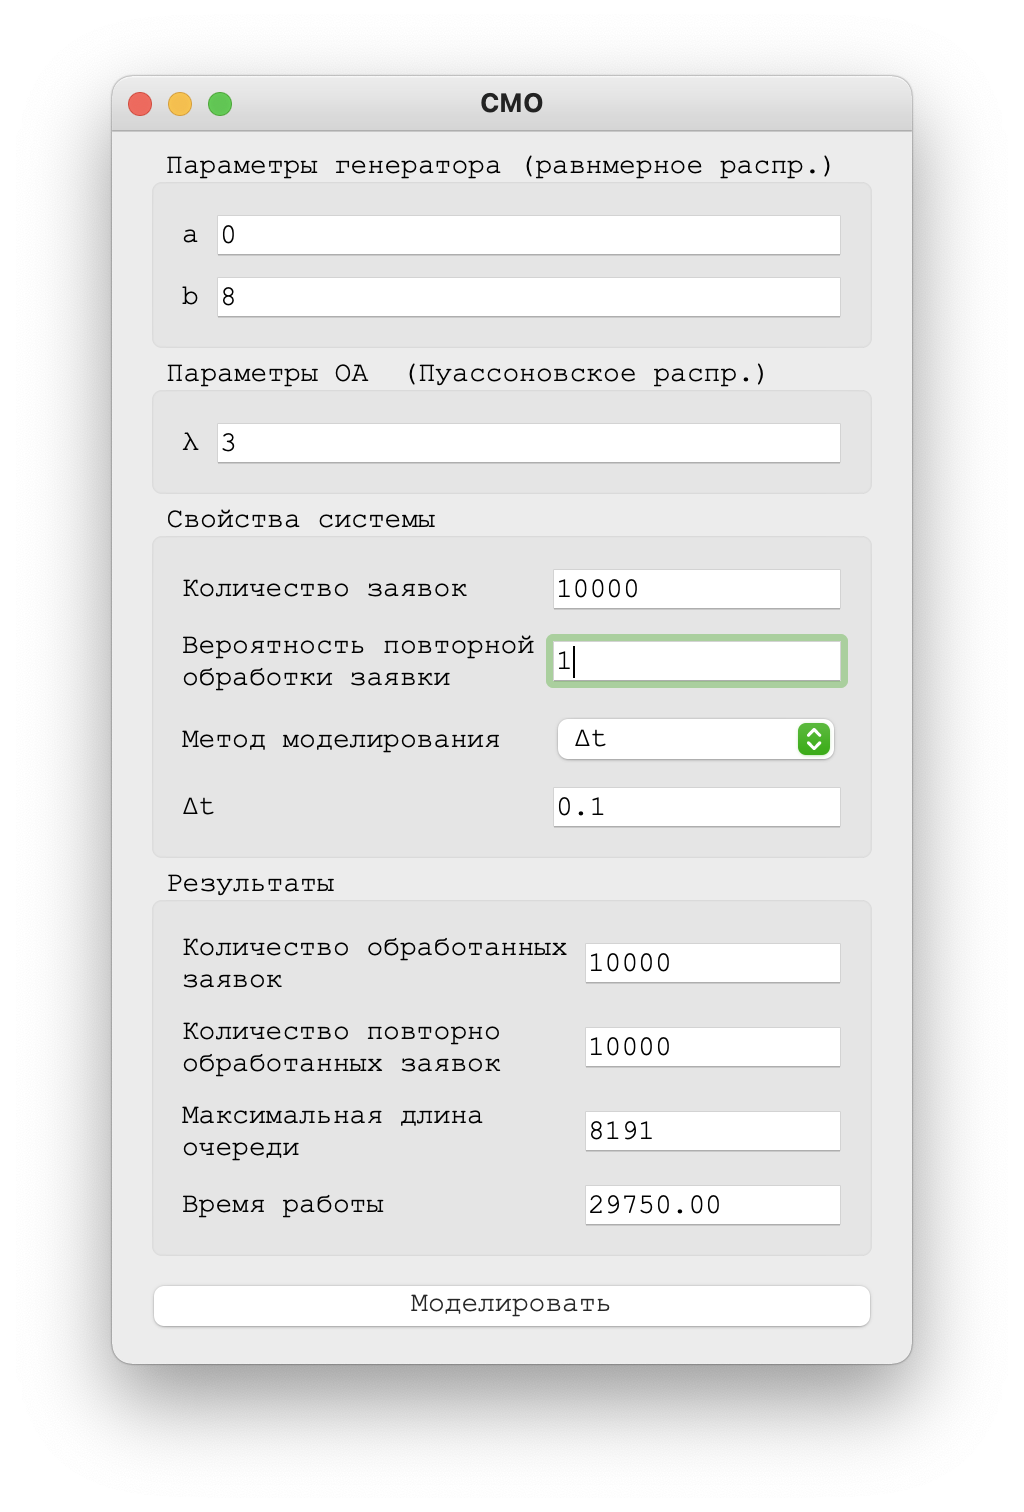
\includegraphics[width=1\linewidth]{3-1-t}
    \end{minipage}
    \caption{Пример работы программы при $p$ = 1 , $\lambda = 3$}
 \end{figure}




 \begin{figure}[!htb]
    \begin{minipage}{0.55\textwidth}
      \centering
      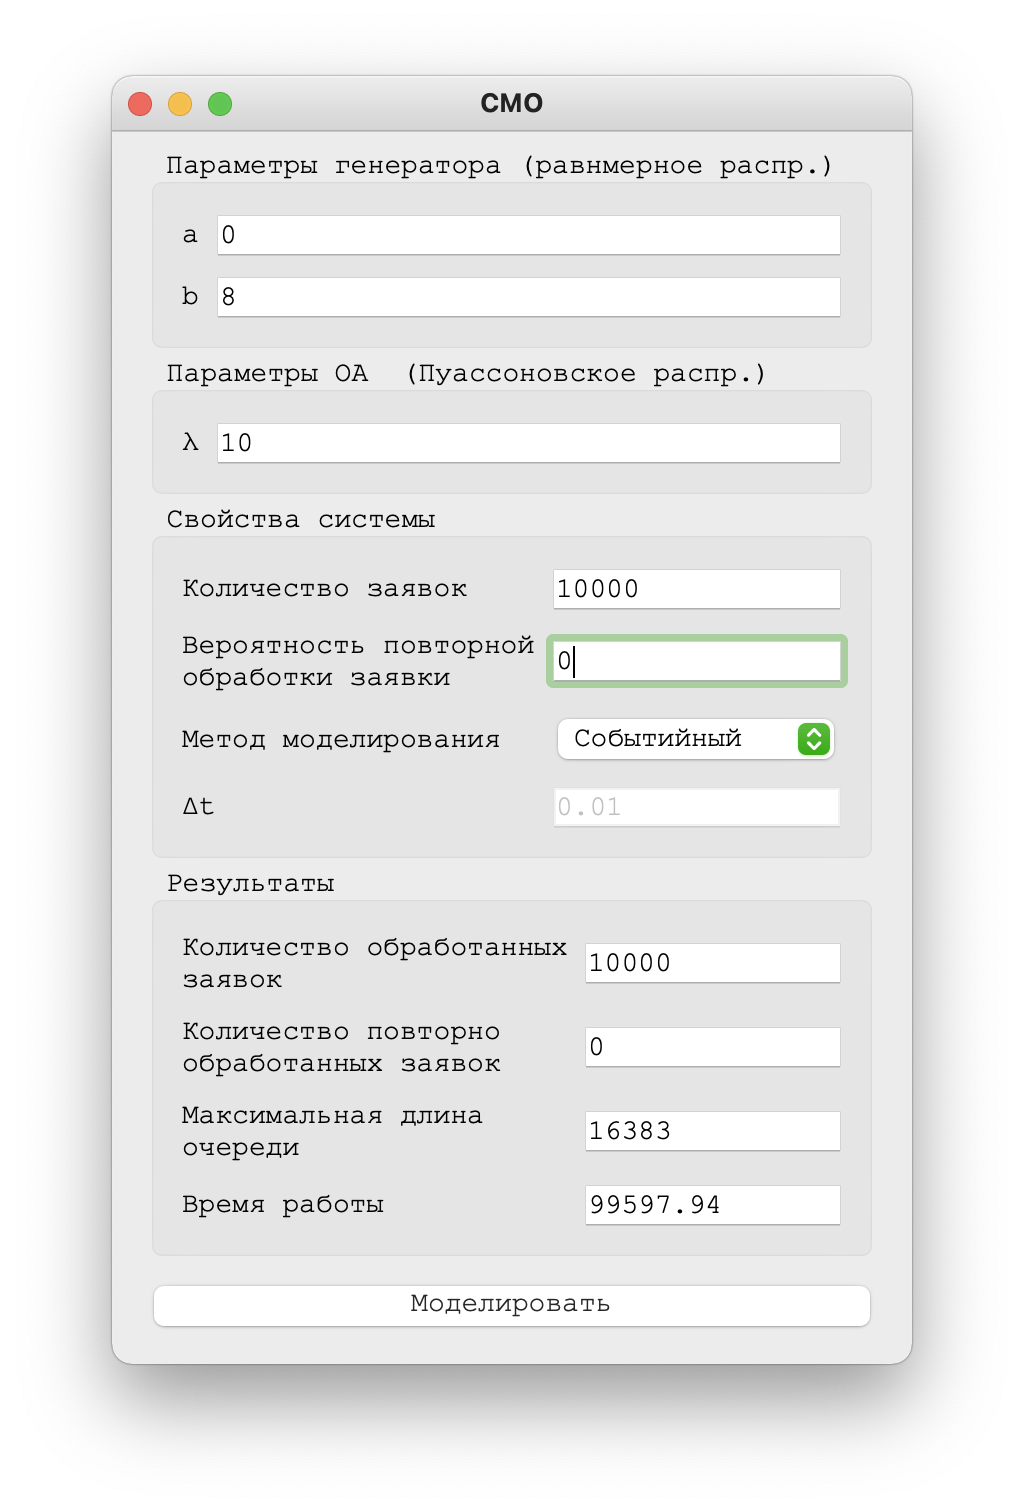
\includegraphics[width=1\linewidth]{10-0-s}
    \end{minipage}\hfill
    \begin{minipage}{0.55\textwidth}
      \centering
      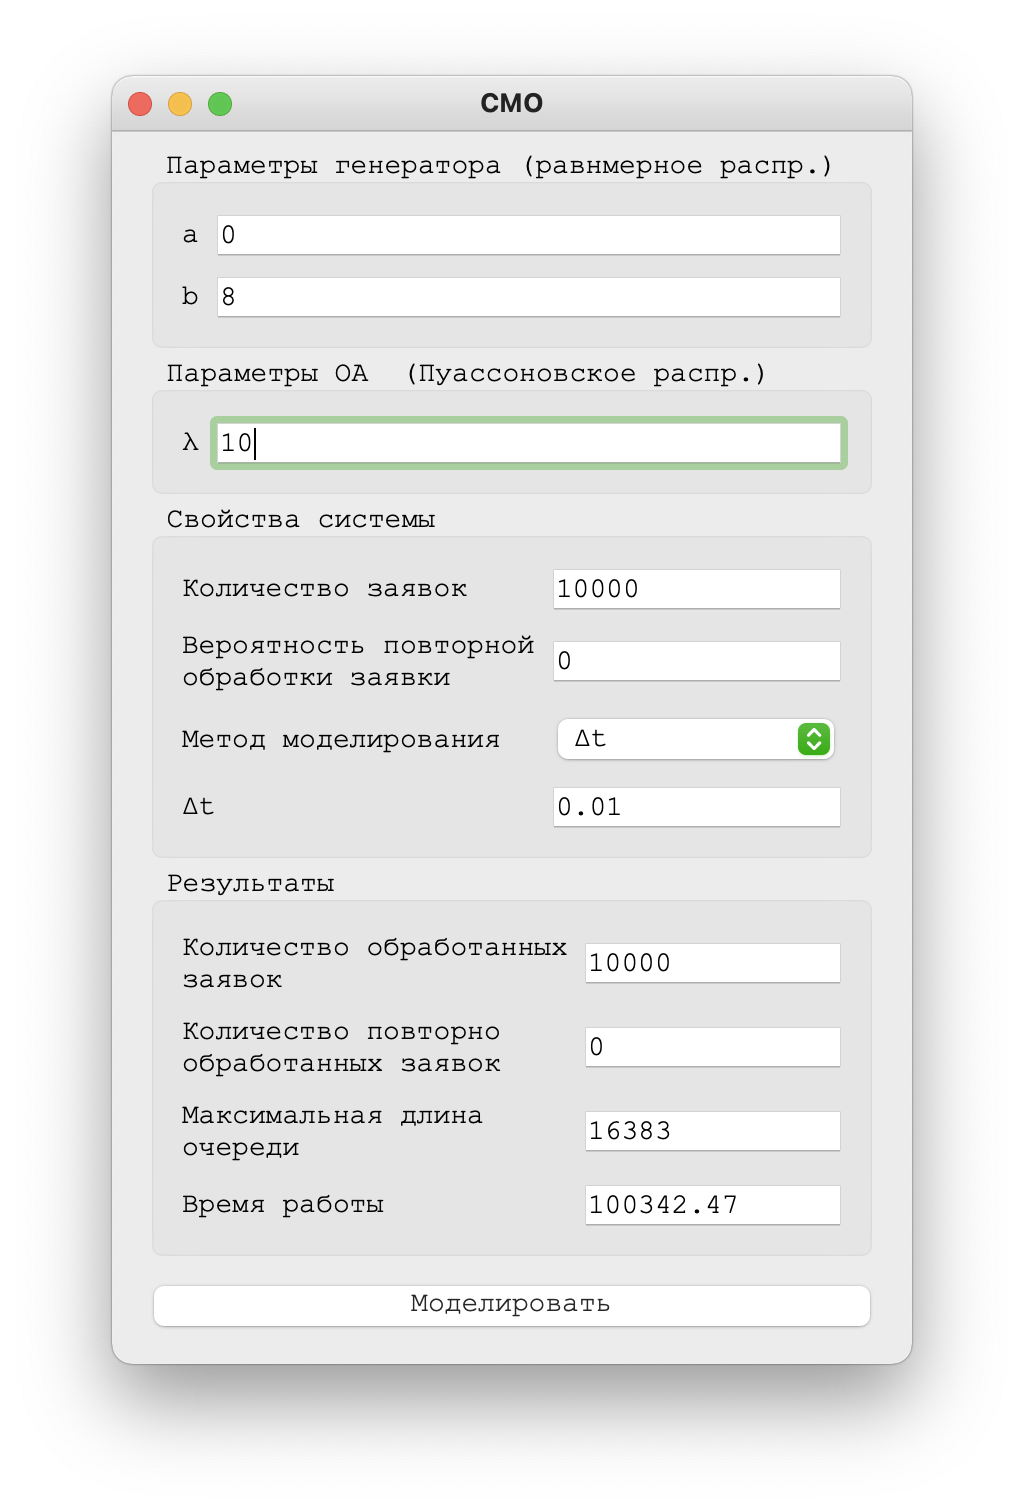
\includegraphics[width=1\linewidth]{10-0-t}
    \end{minipage}
    \caption{Пример работы программы при $p$ = 0 , $\lambda = 10$}
 \end{figure}


 \begin{figure}[!htb]
    \begin{minipage}{0.55\textwidth}
      \centering
      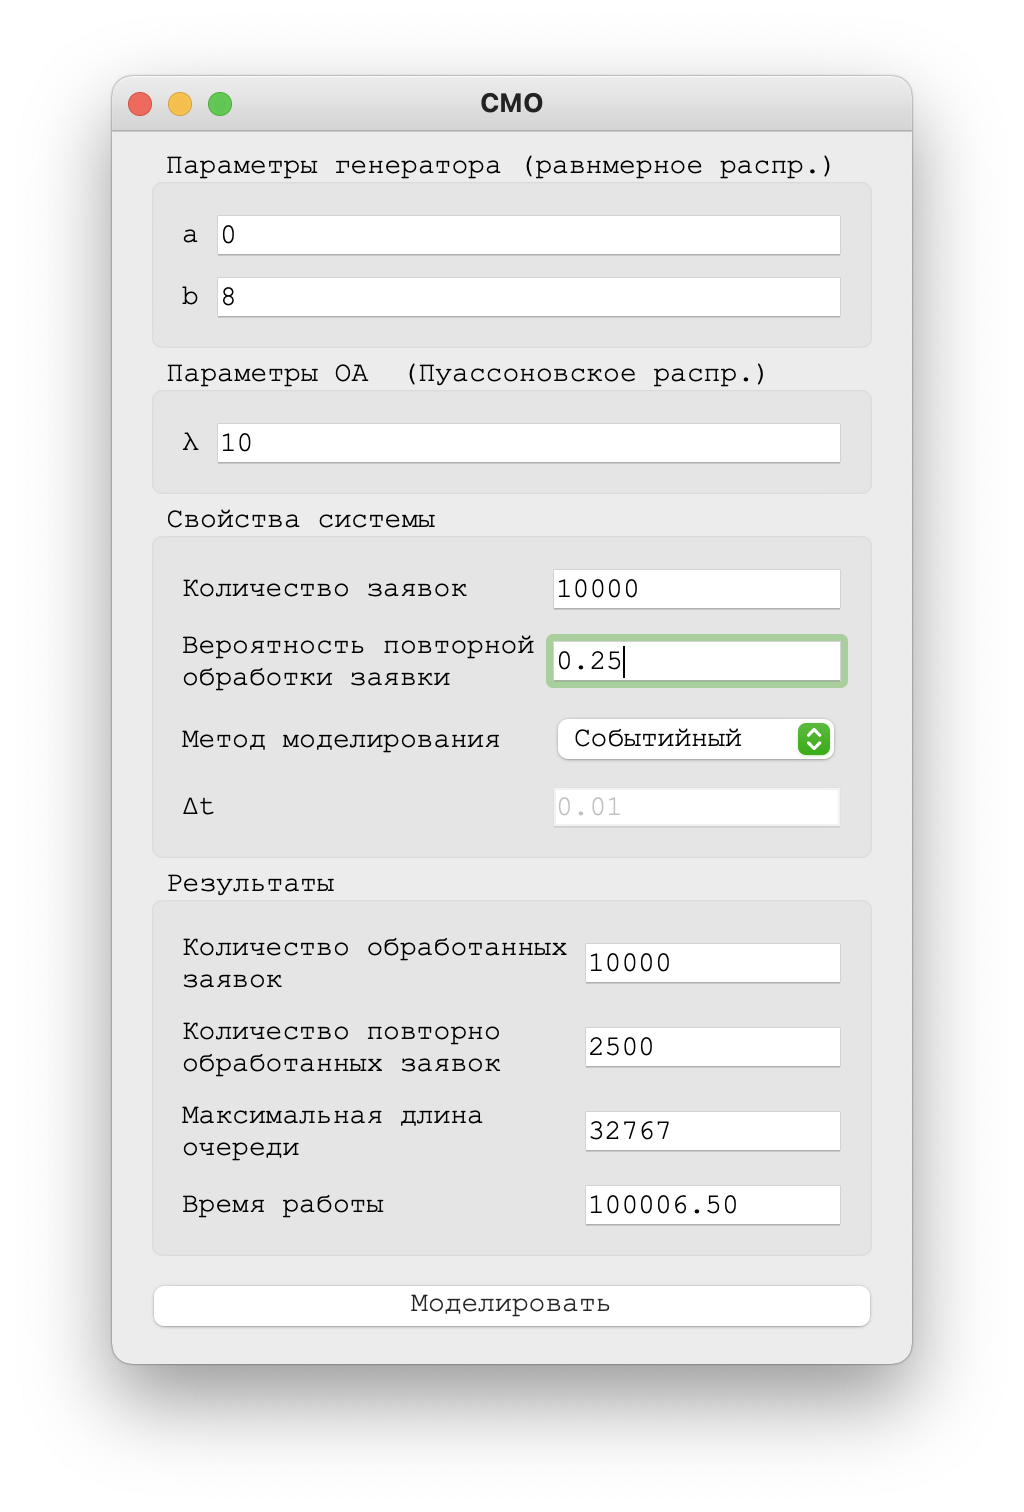
\includegraphics[width=1\linewidth]{10-25-s}
    \end{minipage}\hfill
    \begin{minipage}{0.55\textwidth}
      \centering
      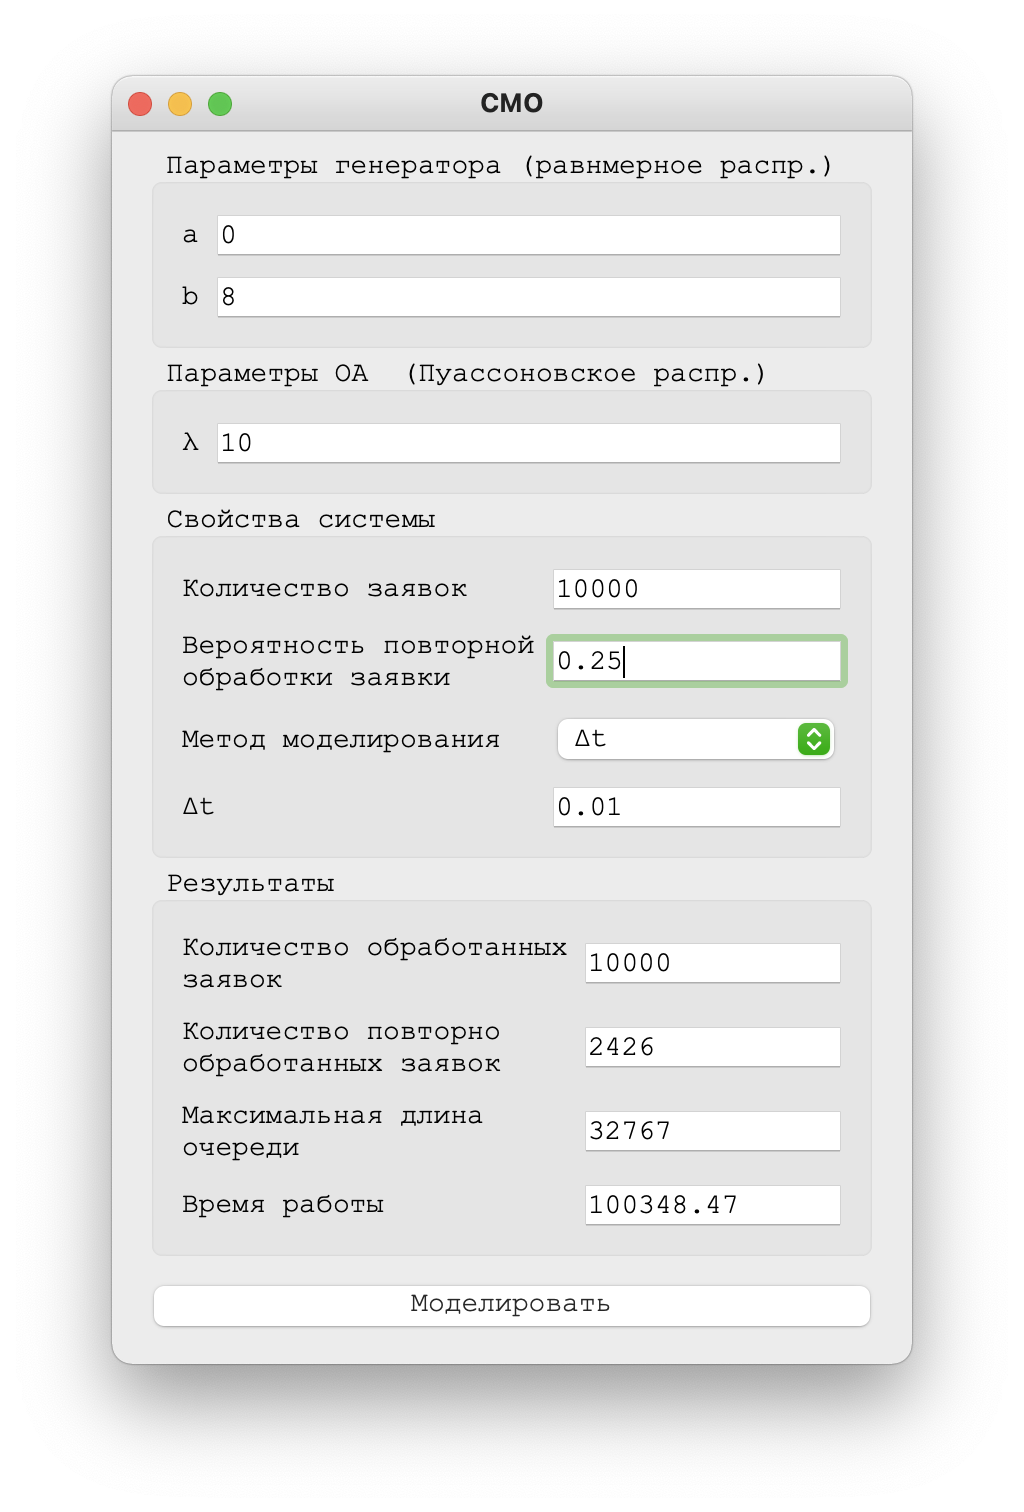
\includegraphics[width=1\linewidth]{10-25-t}
    \end{minipage}
    \caption{Пример работы программы при $p$ = 0.25 , $\lambda = 10$}
 \end{figure}


 \begin{figure}[!htb]
    \begin{minipage}{0.55\textwidth}
      \centering
      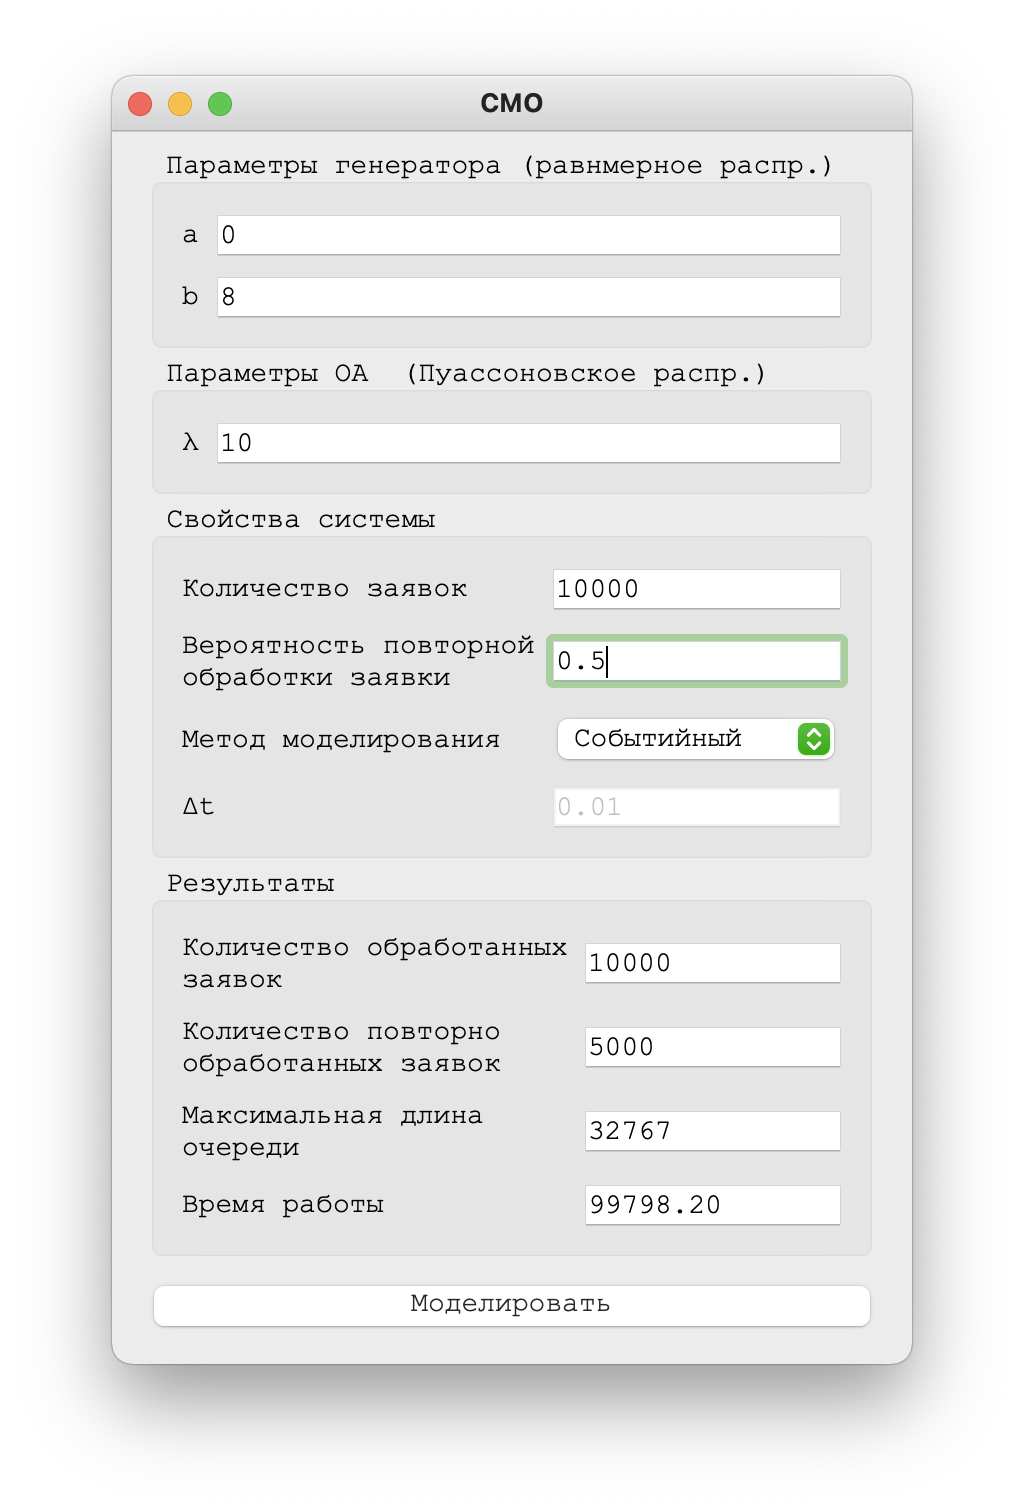
\includegraphics[width=1\linewidth]{10-50-s}
    \end{minipage}\hfill
    \begin{minipage}{0.55\textwidth}
      \centering
      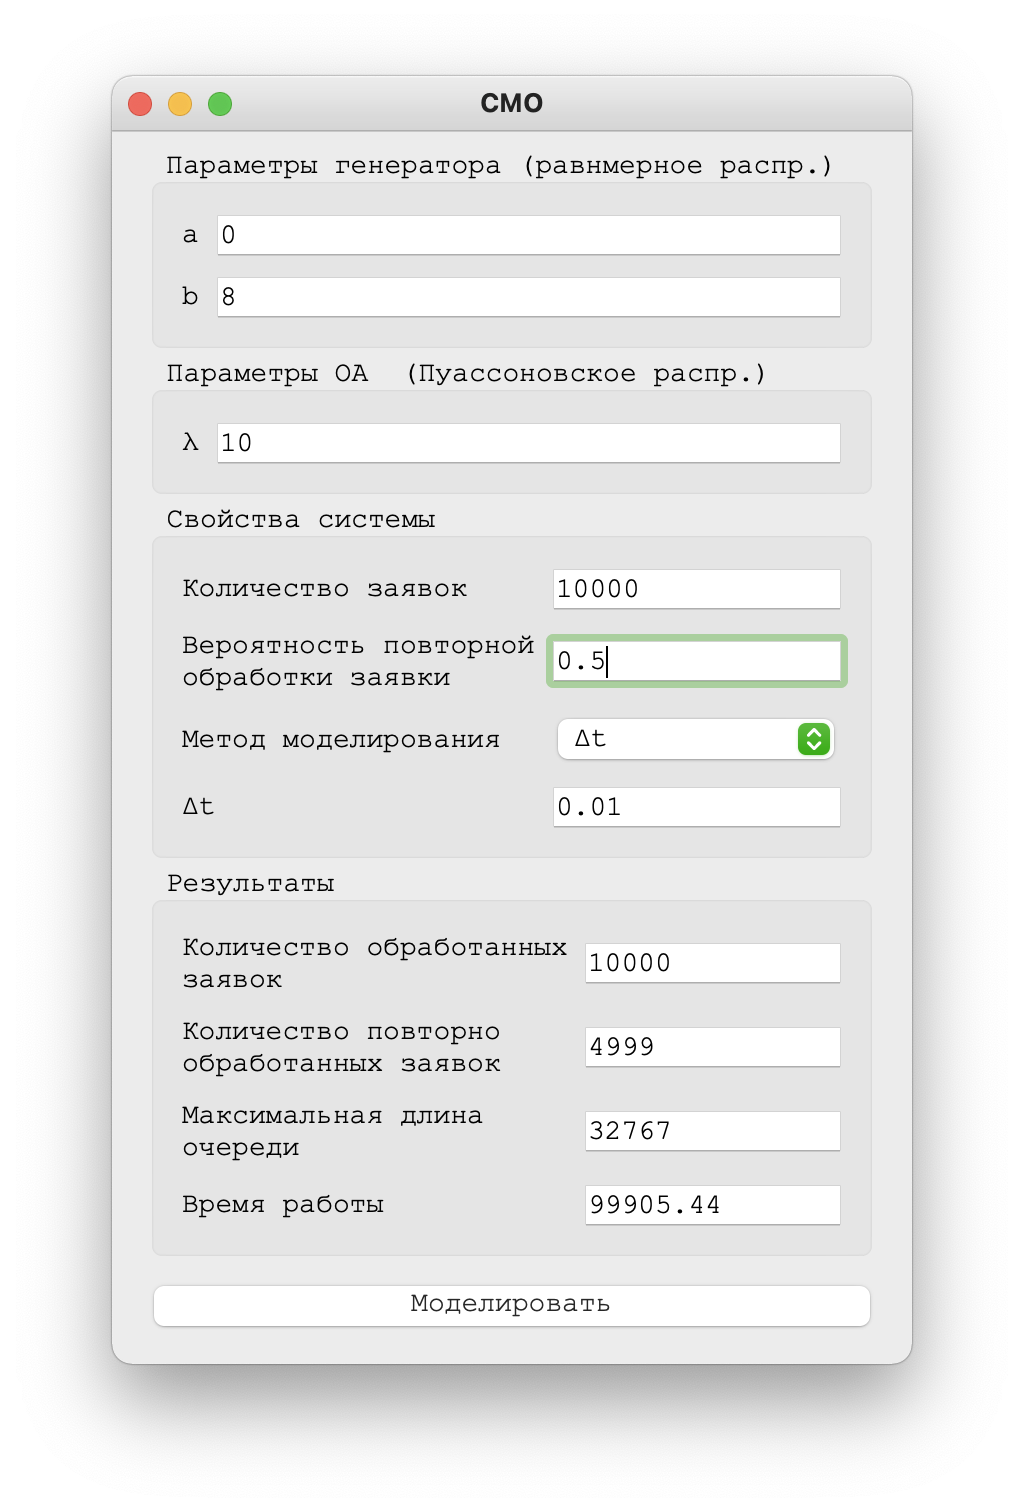
\includegraphics[width=1\linewidth]{10-50-t}
    \end{minipage}
    \caption{Пример работы программы при $p$ = 0.5 , $\lambda = 10$}
 \end{figure}

 
 \begin{figure}[!htb]
    \begin{minipage}{0.55\textwidth}
      \centering
      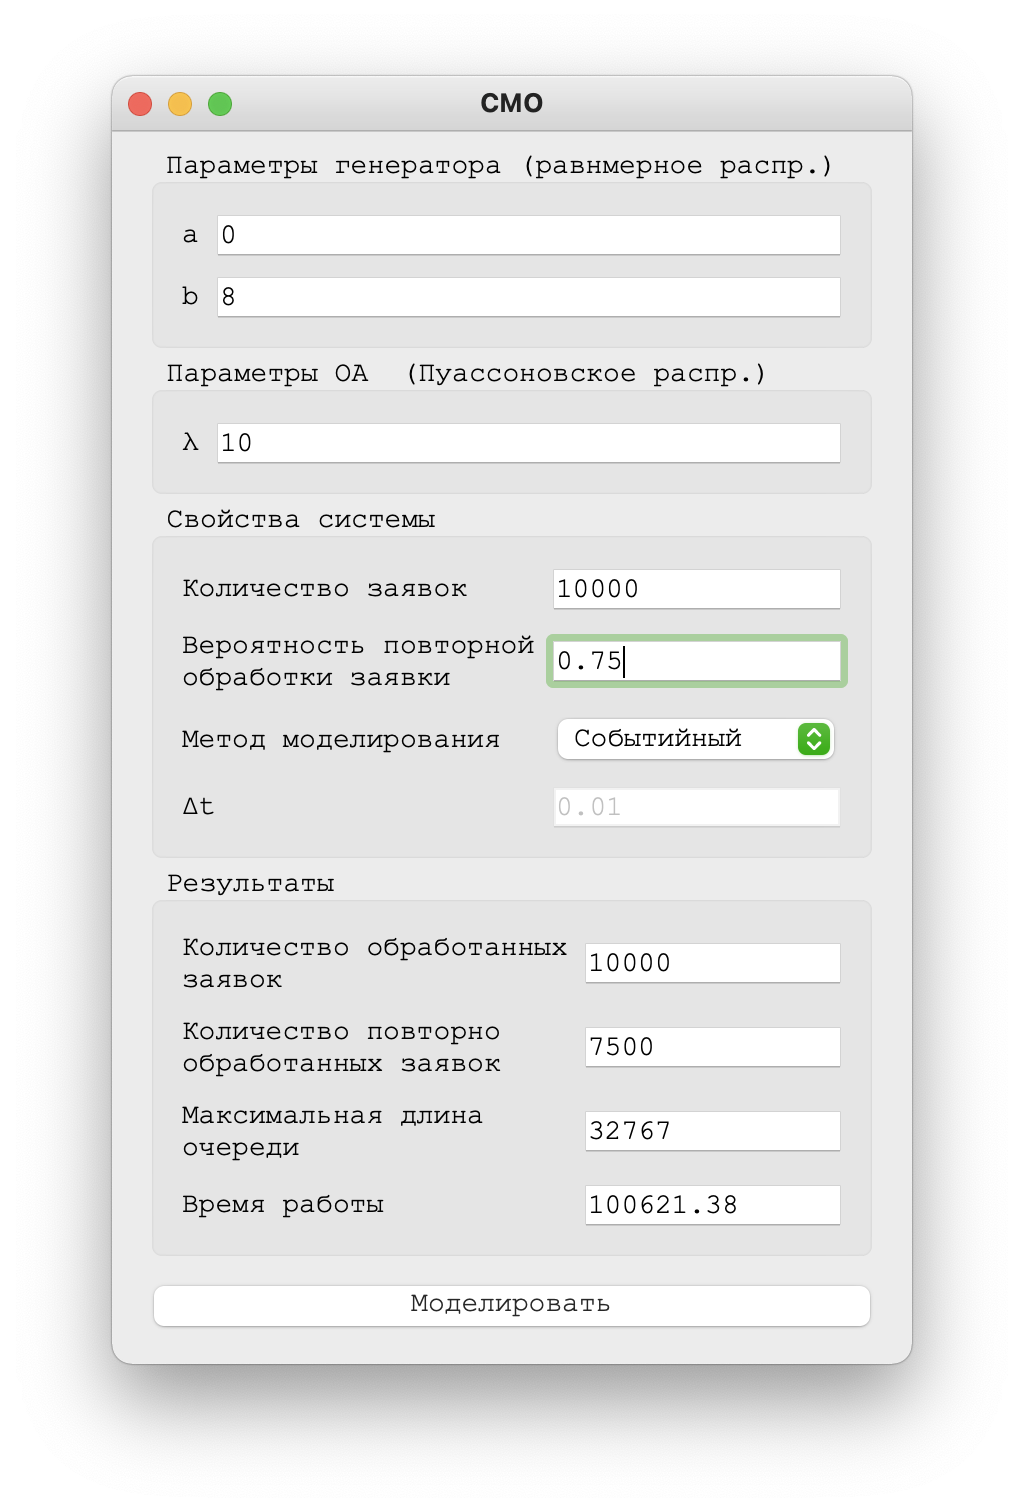
\includegraphics[width=1\linewidth]{10-75-s}
    \end{minipage}\hfill
    \begin{minipage}{0.55\textwidth}
      \centering
      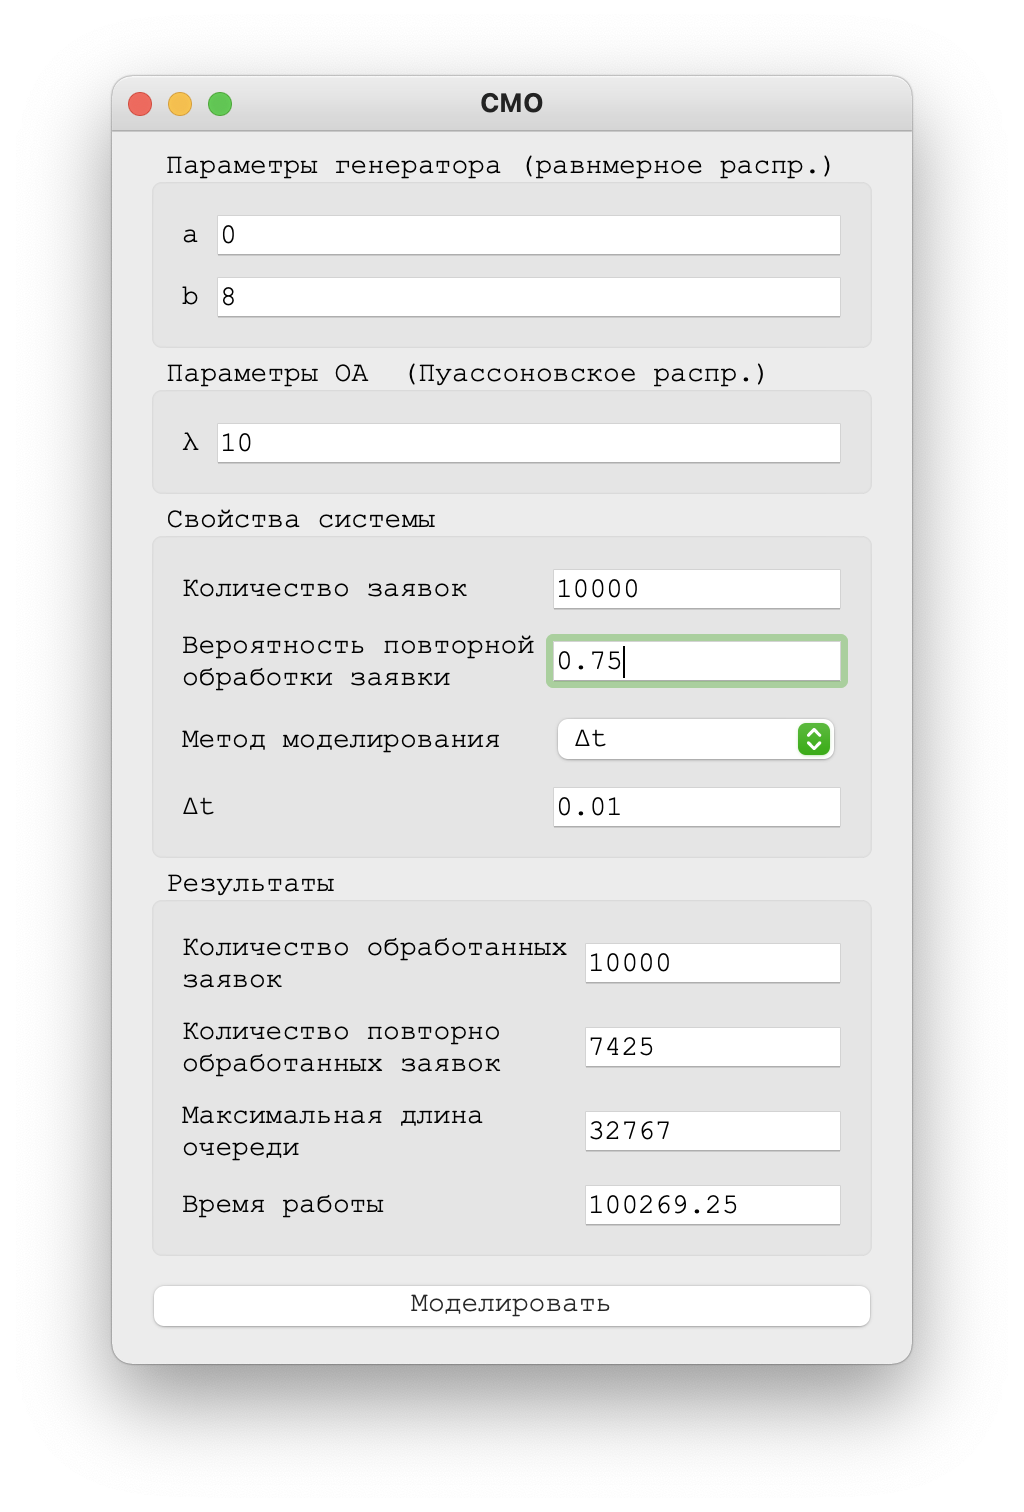
\includegraphics[width=1\linewidth]{10-75-t}
    \end{minipage}
    \caption{Пример работы программы при $p$ = 0.75 , $\lambda = 10$}
 \end{figure}


 \begin{figure}[!htb]
    \begin{minipage}{0.55\textwidth}
      \centering
      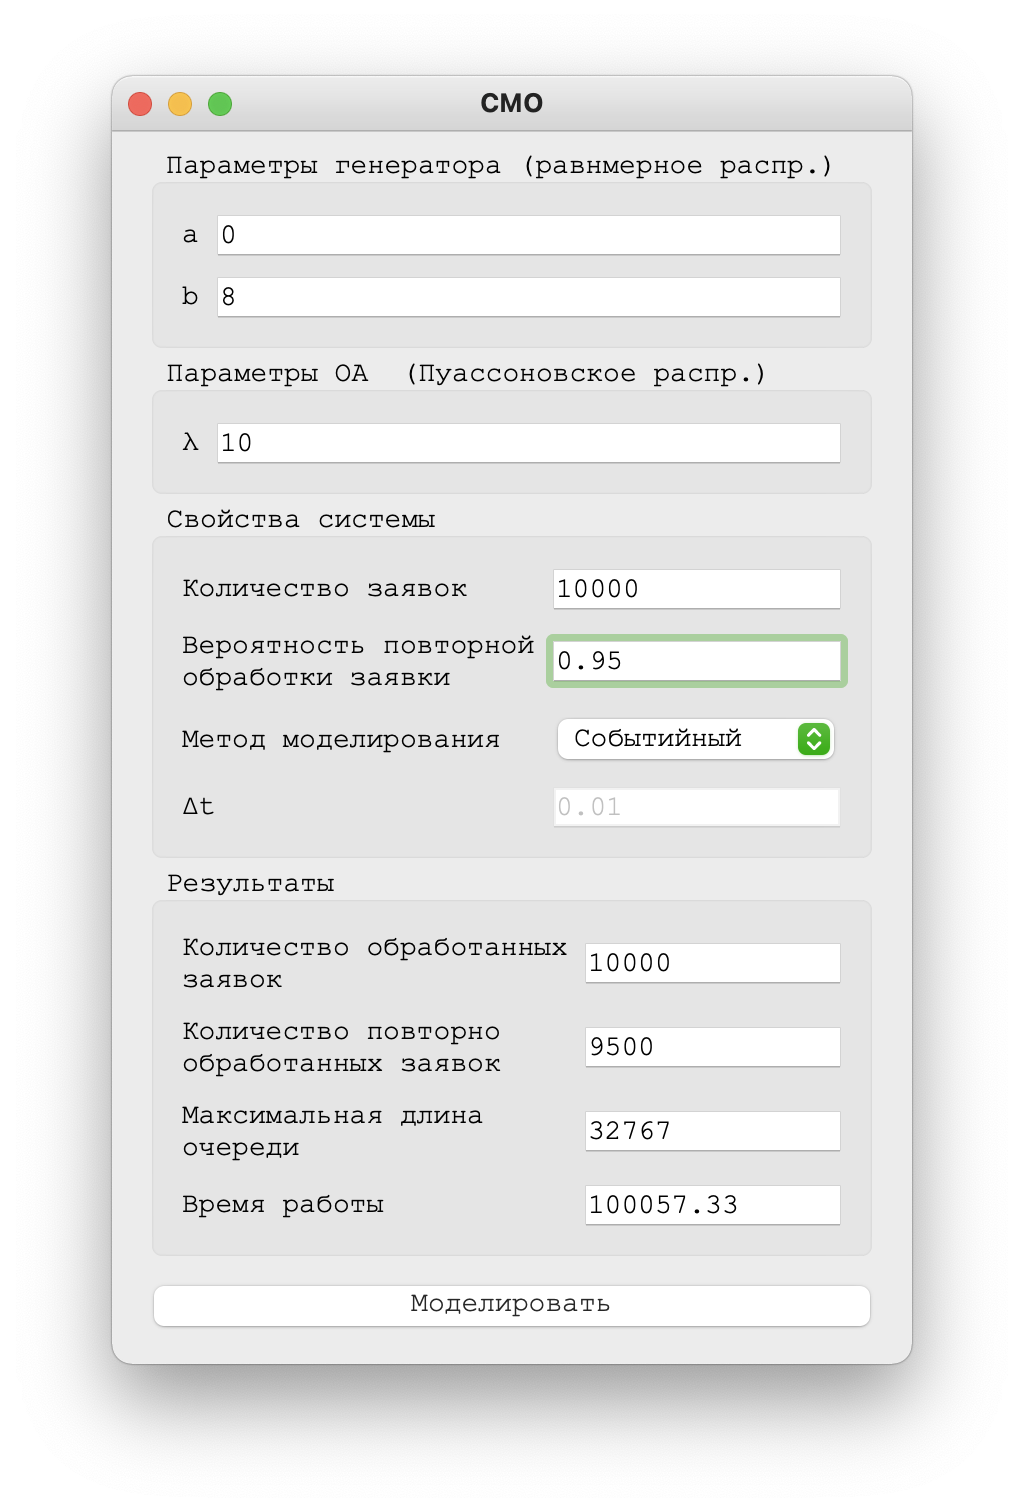
\includegraphics[width=1\linewidth]{10-95-s}
    \end{minipage}\hfill
    \begin{minipage}{0.55\textwidth}
      \centering
      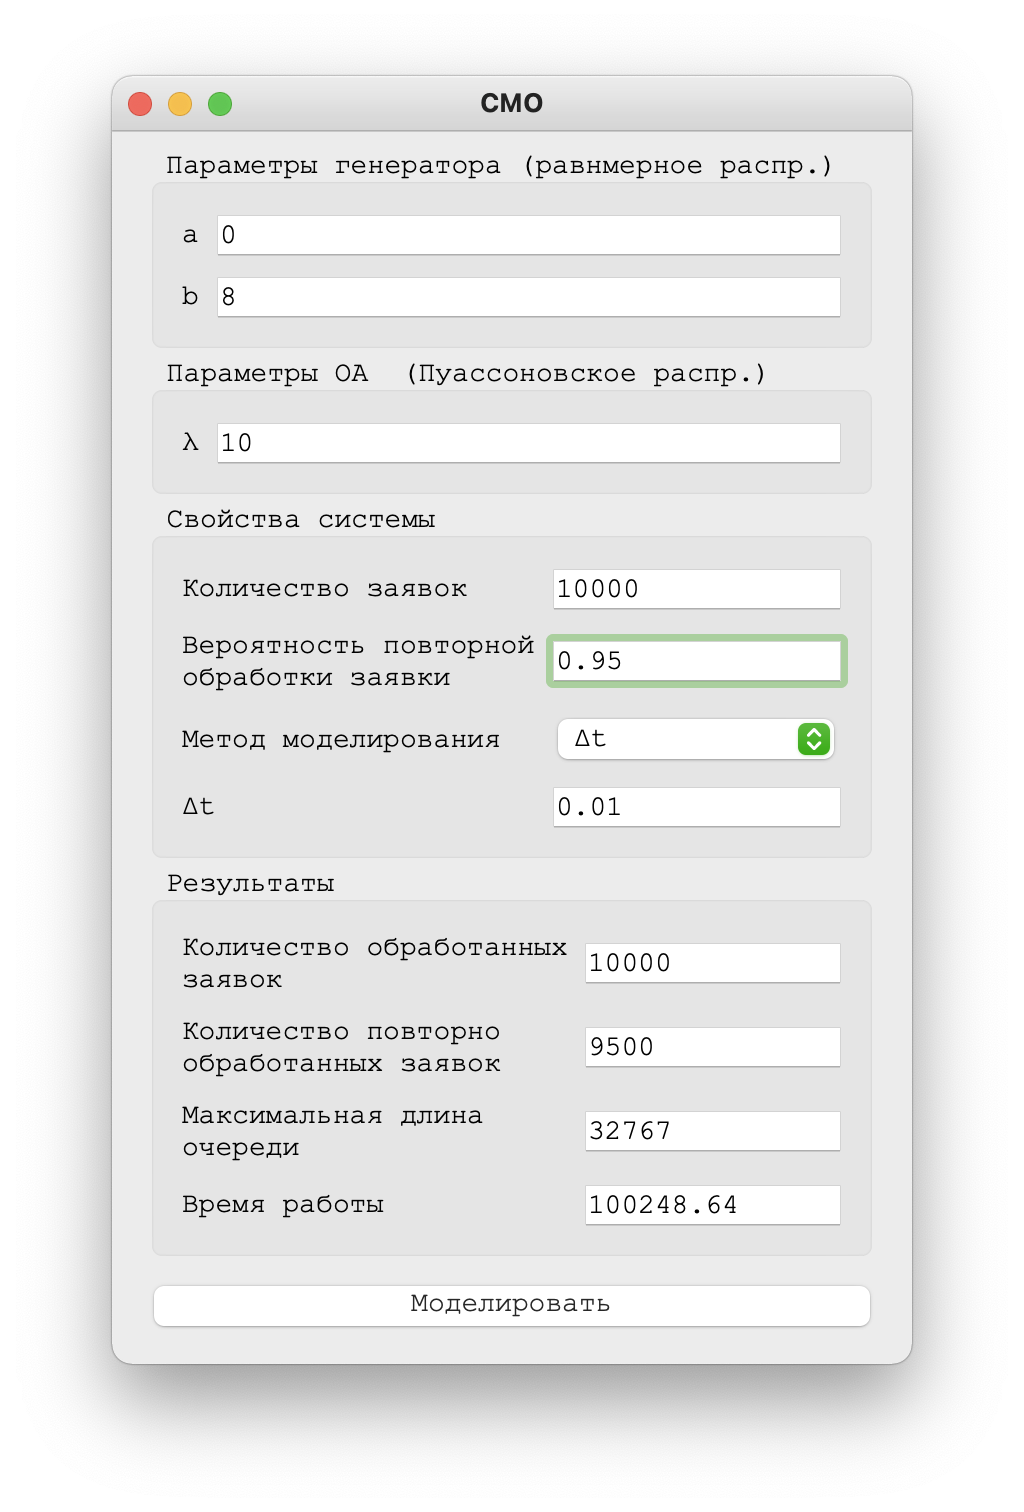
\includegraphics[width=1\linewidth]{10-95-t}
    \end{minipage}
    \caption{Пример работы программы при $p$ = 0.95 , $\lambda = 10$}
 \end{figure}


 \begin{figure}[!htb]
    \begin{minipage}{0.55\textwidth}
      \centering
      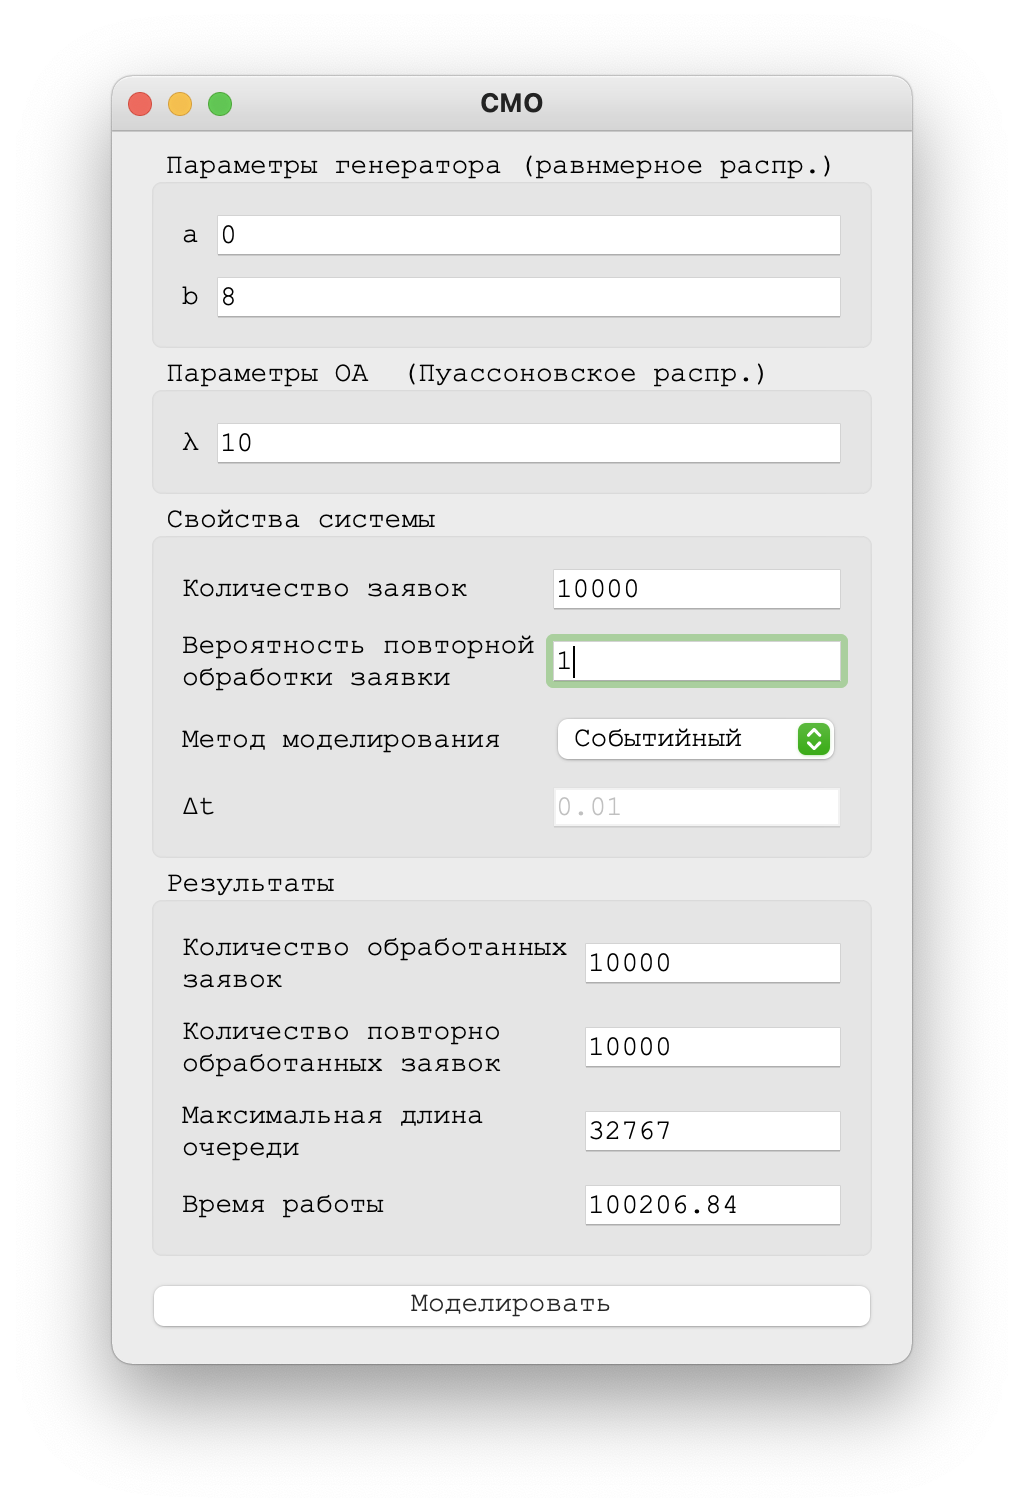
\includegraphics[width=1\linewidth]{10-1-s}
    \end{minipage}\hfill
    \begin{minipage}{0.55\textwidth}
      \centering
      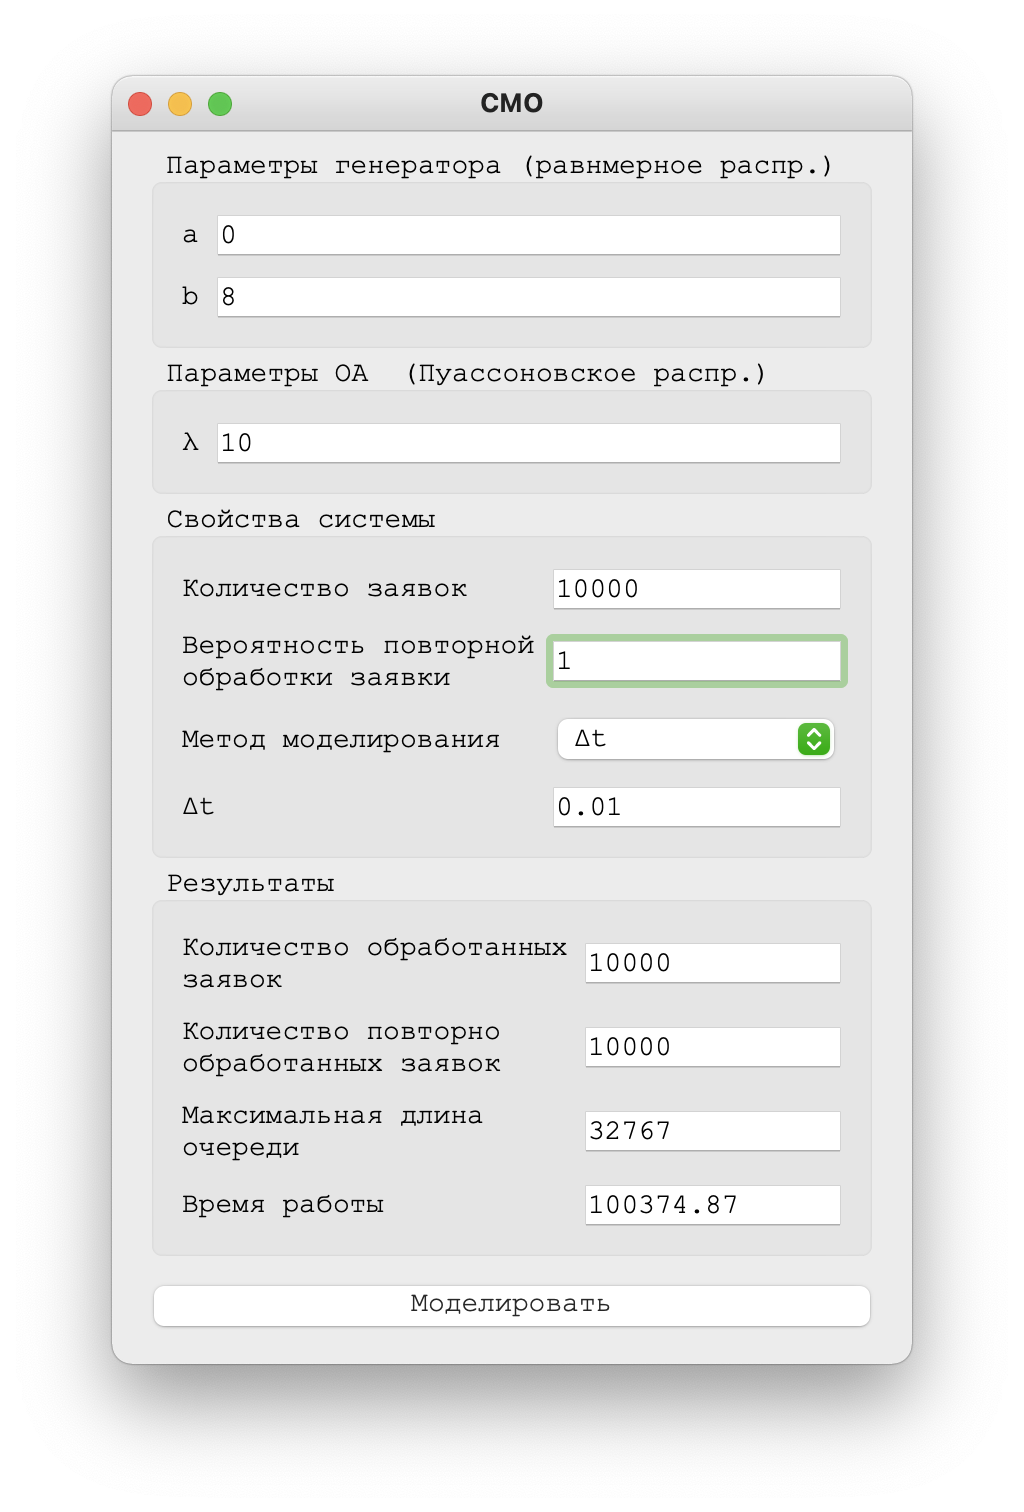
\includegraphics[width=1\linewidth]{10-1-t}
    \end{minipage}
    \caption{Пример работы программы при $p$ = 1 , $\lambda = 10$}
 \end{figure}

 \begin{figure}[!htb]
    \begin{minipage}{0.55\textwidth}
      \centering
      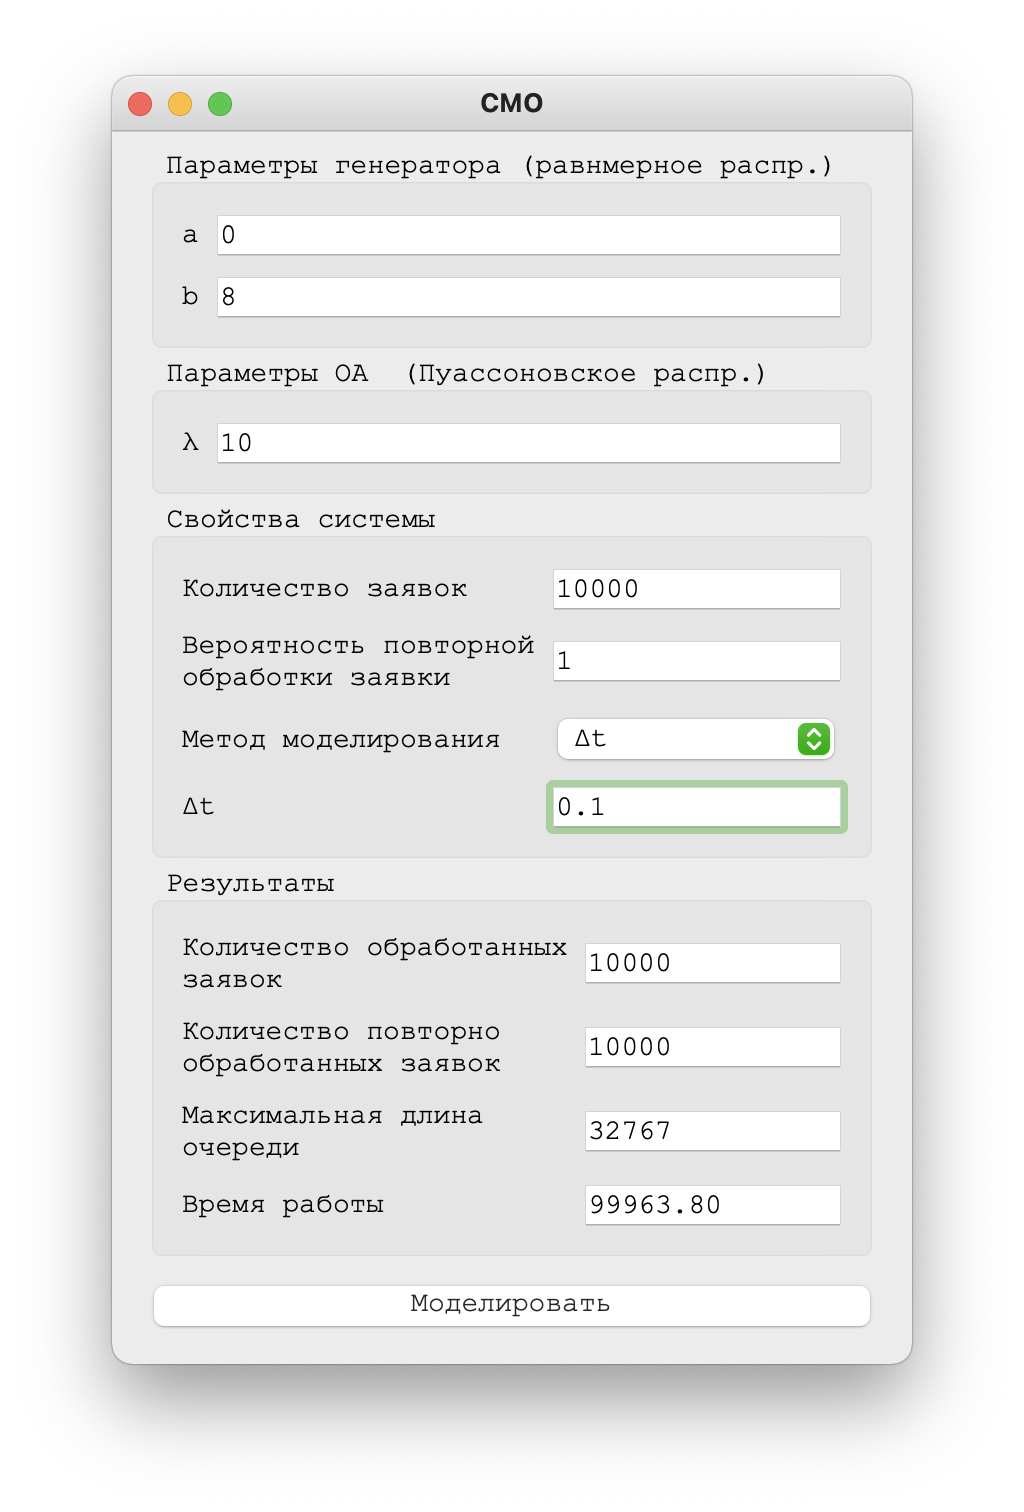
\includegraphics[width=1\linewidth]{10-1-01t}
    \end{minipage}
    \caption{Пример работы программы при $p$ = 1 , $\lambda = 10$, $\Delta t$ = 0.1}
 \end{figure}



% \imgw{170mm}{3-70}{Пример работы программы --  для 3-х разрядных чисел оценки невысокие, т.к. в последовательности из первых разрядов мало уникальных чисел}


\chapter{Код программы}

\lstinputlisting[style=mstyle, caption=modeller.py]{../src/modeller.py}

